\documentclass[runningheads,a4paper,11pt]{llncs}
\usepackage[T1]{fontenc}
\usepackage{pgf}
\usepackage{tikz}
\usetikzlibrary{arrows,automata}
\usepackage[latin1]{inputenc}

% FONTS and SYMBOLS
\usepackage{mathrsfs}
\usepackage{lmodern}
%\usepackage{txfonts}
\usepackage{paralist}

% MATHEMATICS
\usepackage{amsmath,amssymb,amsthm} % AMS packages
%\usepackage[warning, all]{onlyamsmath}

% COLORS and GRAPHICS
\usepackage{graphicx}
\usepackage[left=3cm,right=3cm,top=4cm,bottom=4cm]{geometry}

% FIGURES and TABLES
\usepackage{booktabs} % Better tables

\usepackage{enumerate}
\usepackage{xspace}

\usepackage{microtype} % Prettifies pdf output. Uncomment if you have trouble with this. Will also reduce page count.

%\usepackage[ruled,longend,vlined]{algorithm2e}

\newcommand{\N}{\ensuremath{\mathbf{N}}\xspace} % Natural numbers
\newcommand{\R}{\ensuremath{\mathbf{R}}\xspace}	
% Real numbers
\newcommand{\Z}{\ensuremath{\mathbf{R}}\xspace}	% Integers
\newcommand{\Q}{\ensuremath{\mathbf{Q}}\xspace}	% Fractions
\renewcommand{\cal}{\mathcal}

\newcommand{\pr}{\ensuremath{\mathbf{Pr}}}
\newcommand{\PR}[2]{\ensuremath{\mathbf{Pr}_{#1} \left [ #2 \right ]}}
\newcommand{\ex}{\ensuremath{\mathbf{E}}}
\newcommand{\EX}[2]{\ensuremath{\mathbf{E}_{#1} \left [ #2 \right ]}}
\newcommand{\mat}[1]{\ensuremath{\boldsymbol{#1}}}
\newcommand{\vect}[1]{\ensuremath{\boldsymbol{#1}}}
\newcommand{\bvect}{\ensuremath{\boldsymbol{B}}}
\newcommand{\trans}[1]{\ensuremath{{#1}^{\scriptscriptstyle \mathsf{T}}}}
\newcommand{\norm}[1]{\ensuremath{\left \| #1 \right \|}}
\newcommand{\normsq}[1]{\ensuremath{\left \| #1 \right \|^2}}
\newcommand{\pseudo}[1]{\ensuremath{{#1}^{+}}}
\newcommand{\inv}[1]{\ensuremath{{#1}^{-1}}}
\newcommand{\etal}{\emph{et al.\!}}
\renewcommand{\th}{\ensuremath{^{\textrm{th}}}}
\renewcommand{\epsilon}{\varepsilon}

\newtheorem{lemma}{Lemma}
\newtheorem{theorem}{Theorem}
\newtheorem{corollary}{Corollary}
\newtheorem{observation}{Observation}
\newtheorem{proposition}{Proposition}

\theoremstyle{definition}
\newtheorem{definition}{Definition}

%\usepackage[left=3cm,right=3cm,top=3cm,bottom=3cm]{geometry}

\usepackage{authblk}
%\usepackage{cleveref}
\pagestyle{plain}
\title{Overlapping Communities in Social Networks\thanks{Research 
funded by DFG Project RO 927/13-1 ``Pragmatic Parameterized Algorithms.''}}
\author{Jan Dreier, 
Philipp Kuinke, 
Rafael Przybylski,
Felix Reidl, 
Peter Rossmanith, 
Somnath Sikdar
}

\institute{Theoretical Computer Science, \\ 
RWTH Aachen University, \\
52074 Aachen Germany}


\begin{document}
\maketitle

\begin{abstract}
Complex networks can be typically broken down into sets of vertices that are
more densely connected on the inside than outside. Discovering this ``community
structure'' is an important step in studying the large-scale structure of
networks. Many algorithms have been proposed for community detection and
benchmarks have been created to evaluate their performance. Typically algorithms
for community detection either find a partition of the node set of the graph
(non-overlapping communities) or find a collection of sets that cover the entire
node set (overlapping communities). 

In this paper, we propose a particularly simple semi-supervised learning
algorithm for finding out communities. In essence, given the community
information of a small number of \emph{seed nodes}, the method uses random walks
from the seed nodes to uncover the community information of the remaining
network.  The algorithm runs in time $O(k \cdot m \cdot \log n)$, where $m$ is
the number of edges; $n$ the number of nodes; and $k$ the number of communities
in the network.  In sparse networks with $m = O(n)$ and a constant number of
communities, this running time is almost linear in the size of the network.
Another important feature of our algorithm is that it can be used for either
non-overlapping or overlapping communities. 

We test our algorithm using the LFR benchmark created by Lancichinetti,
Fortunato, and Radicchi~\cite{LFR08} specifically for the purpose of evaluating
such algorithms. Our algorithm can compete with the best of algorithms for both
non-overlapping and overlapping communities as found in the comprehensive study
of Lancichinetti and Fortunato~\cite{LF09}. Some of the algorithms in that study
include several variants of the well-known modularity maximization approach,
which takes $O(n^2)$ time on sparse graphs~\cite{RCC04}; clique detection
algorithms such as Cfinder which takes exponential time in the worst
case~\cite{PDFV05}; techniques based on random walks such as the Infomap method
which reportedly perform well in practice but whose  worst-case running times
have not been reported~\cite{RB08}. 

\end{abstract}

\section{Introduction}
Many real-world graphs that model complex systems exhibit an organization 
into subgraphs, or \textit{communities} that are more densely connected on the inside than between each other. 
Social networks such as Facebook and LinkedIn divide into groups of friends 
or coworkers, or business partners; scientific collaboration networks divide 
themselves into research communities; the World Wide Web divides into groups 
of related webpages. The nature and number of communities provide 
a useful insight into the structure and organization of networks. 

Discovering the community structure of networks is an 
important problem in network science and is the subject 
of intensive research~\cite{GN02, GN04, CNM04, RCC04, DM04, PDFV05, NL07, 
BGLL08, RB08, RN09}. Existing community detection algorithms are 
distinguished by whether they find partitions of the node set 
(non-overlapping communities) or node covers (overlapping communities). 
Typically finding overlapping communities is a much harder problem and most of the 
earlier community detection algorithms focused on finding disjoint 
communities. A comparative analysis of several community detection algorithms 
(both non-overlapping and overlapping) was presented by Lancichinetti and Fortunato 
in~\cite{LF09}. In this paper we closely follow their test framework, 
also called the LFR-benchmark.

The notion of a community is a loose one and currently there is no 
well-accepted definition of this concept. A typical approach is to consider 
a partition of the node set such that the density of the edges within a partite 
set (intra-community edges) is greater than the density of edges across partitions 
(inter community edges). Various community detection algorithms formalize this
idea differently. One of the very first algorithms by
Girvan and Newman~\cite{GN02} introduced a measure known as \textit{modularity}
which, given a partition of the nodes of the network, compares the fraction of 
inter-community edges with the edges that would be present had they been 
rewired randomly preserving the node degrees. Other authors such as Palla 
\etal~\cite{PDFV05} declare communities as node sets that formed 
by overlapping maximal cliques. Rosvall and Bergstrom~\cite{RB08} 
define the goodness of a partition in terms of the number of bits required to 
describe per step of an infinite random walk in the network, the intuition being 
that in a ``correct'' partition, a random walker is likely to spend more time 
within communities rather than between communities, thereby decreasing the 
description of the walk.  

A severe restriction of many existing community detection algorithms 
is that they are too slow. Algorithms that optimize modularity typically 
take $O(n^2)$, even on sparse networks. The overlapping clique finding 
algorithm of Palla \etal~\cite{PDFV05} take exponential time in the worst case.
In other cases, derivation of worst-case running time bounds are ignored. 

\paragraph{Our contribution.}
Given that it is unlikely that users of community detection algorithms 
would unanimously settle on one definition of what constitutes a community, 
we feel that existing algorithms ignore the \emph{user perspective}.
To this end, we chose to design an algorithm that takes the network structure, 
as well as user preferences into account. 
The user is expected to classify a small set of nodes of the network 
into communities (which may be 6--8\% of the nodes of each community).
Obviously this is possible only when the user has some 
information about the network, such as, what it represents, which nodes 
are the important ones and into which communities they are classified. 

Such situations are actually quite likely. The user might have data only 
on the leading scientific authors in a co-authorship network 
and would like to find out the research areas of the remaining members of the network. 
He may either be interested in a broad partition of the network into into its main fields
or a fine grained decomposition into various subfields.
By labeling the known authors accordingly,
the user can specify which kind of partition he is interested in.
Another example would be the detection of trends in a social network.
Consider the case where one knows the political affiliations of some people 
and aims to discover political spectrum of the whole network, 
for example, to predict the outcome of an election. 


Another scenario where this may be applicable is in recommendation systems. 
One might know the preferences of some of the users of an online retail 
merchant possibly because they purchase items much more frequently than others. 
One could then use this in the network whose nodes consist of users, with two 
nodes connected by an edge if they represent users that had purchased similar products in the past. 
The idea now would be to use the knowledge of the prefererences of a few to 
predict the preferences of everyone in the network. 
\texttt{Movie database example?}


An important characteristic of algorithms surveyed in~\cite{LF09} 
is that the algorithms either find disjoint communities or overlapping 
ones. Most algorithms solve the easier problem of finding disjoint communities. 
The ones that are designed to find overlapping communities such as the overlapping clique finding 
algorithm of Palla \etal~\cite{PDFV05} do not seem to yield very good results (see~\cite{LF09}).
Our algorithm naturally extends to the overlapping case. Of course, there is a higher 
price that has to be paid in that the number of nodes that need to be classified by the user 
typically is larger (5\% to 10\% of the nodes per community). The algorithm, however,
does not need any major changes and we view this is as an aesthetically pleasing 
feature of our approach. 

Thirdly, in many other approaches, the worst-case running time of the algorithms 
is neither stated nor analyzed. We show that our algorithm runs in time $O(k \cdot m \cdot \log n)$, 
where $k$ is the number of communities to be discovered (which is supplied by the user), 
$n$ and $m$ are the number of nodes and edges in the network. In the case of sparse graphs 
and a constant number of communities, the running time is $O(n \cdot \log n)$. Given that even 
an $O(n^2)$ time algorithm is too computationally expensive on many real world graphs, 
a nearly linear time algorithm often is the only feasible solution.   

Finally, we provide an extensive experimental evaluation of our algorithm on the LFR benchmark
introduced by Lancichinetti, Fortunato and Radicchi in~\cite{LFR08, LF09}. In order to ensure 
a fair comparison with other algorithms reviewed in~\cite{LF09}, 
we choose all parameters of the benchmark as in the original paper.


This paper is organized as follows. In Section~\ref{sec:major_algorithms}, we review some 
of the more influential algorithms in community detection. In Section~\ref{sec:algorithm}, we 
describe our algorithm and analyze its running time. In Sections~\ref{sec:experiment_setup} 
and~\ref{sec:experiment_results}, we present our experimental results. Finally we conclude 
in Section~\ref{sec:conclusions} with possibilities of how our approach might be extended. 





\section{The Algorithm} \label{sec:algorithm}
A \emph{social network} consists of a set of social actors and a set of ties 
between them. A social network is modeled as a graph which may be directed 
or undirected. In this paper, we deal with social networks that are modeled as undirected 
graphs. In the context of community detection in social networks, we make 
the following assumptions. 

Our first assumption is that we know what the network at hand represents. That is, 
we have a sense of context about the network. The network could represent 
friendships as in the Facebook network; co-authorships as in the DBLP network; 
it could be a network of professionals such as LinkedIn, or a network of movie 
lovers such as IMDB. Secondly, we assume that we know what is it that constitutes 
a community within the network. This is crucial because, for one, we do not 
formally define what a community is. We take it as being given as part of the 
input specification. While this may appear as an artifice, in many real-life situations 
where we are required to find communities, we do in fact know what 
it is that we are searching for. For example, we might want to find the set of 
people with a given political leaning, or a set of people who love a particular 
genre of movie, or a set of people with a specific skill-set and experience. 
In each of these cases, we have a sense of what it is that is required to be found. 

In broad brush-strokes, this is how our algorithm works.  It requires that we know
some members from each community that we are aiming to discover. We call these members 
\emph{seed nodes}. A seed node can belong to several communitites and our algorithm 
actually finds out overlapping communities in the network. The algorithm uses the 
partial community information and propagates it to the other nodes of the network 
by simulating a random walk from non-seed nodes to the set of seed nodes. 

Suppose that $x_1, \ldots, x_s$ are the seed nodes in the network and that a random walk starting at 
a non-seed node~$u$ reaches these nodes with probabilities $p_1, \ldots, p_s$. If out 
of these~$s$ seed nodes, $x_{i_1}, \ldots, x_{i_r}$ belong to a community~$C$, then 
the algorithm assigns a probability of $\sum_{j = 1}^r p_{i_j}$ for the event 
that~$u$ belongs to~$C$. For each community, we can now assign a probability for 
the event that~$u$ belongs to it. The communities that the algorithm 
assigns~$u$ are those for which the probabilities exceed a certain threshold. 

The random walk can be represented by a transition matrix and the walk itself can be simulated 
by multiplying this matrix with itself repeatedly. This, however, takes $O(n^3)$
time, where~$n$ is the number of nodes in the network. One of the contributions of 
this paper is to show how this can be reduced to solving a set of Laplacian system 
of linear equations (one set per seed node), which by the work of Speilman and 
Teng~\cite{Vis13} can be done in $O(m \log n)$ time, where~$m$ is the number of edges
in the graph. We assume that our networks are sparse in the sense that $m = O(n)$, 
so that the running time of our algorithm can  be bounded by $O(s n \log n)$.    
        
\subsection{Absorbing Markov Chains and Random Walks}
We now provide a formal description of our model. We assume that our network 
is a simple undirected graph $G = (V,E)$ with~$n$ nodes and~$m$ edges, where $m = O(n)$.
We also know that there are~$k$ communities which may overlap in an arbitrary fashion.
In practical situations, we have~$k \ll n$. 
Moreover, we have some partial information about each community in that we know
$\log n$ members of each community. Call such members of the network \emph{seed nodes} 
and the remaining nodes \emph{non-seed nodes}. Together, we know the community information 
of $k \cdot \log n$ seed nodes. The community information of a node~$u$ is represented 
by a $1 \times k$ vector called the \emph{affinity vector} of~$u$, denoted 
by 
\[
	\bvect (u) = \left ( \alpha (u, 1), \ldots, \alpha (u, k) \right ).
\] 
The entry $\alpha (u, i)$ of the belonging vector represents the probability that 
node~$u$ belongs to community~$i$.  We call this the \emph{affinity of node~$u$} for 
community~$i$. We point out that $\sum_{i = 1}^k \alpha (u, i)$ 
need not be~$1$. An example of this situation is when~$u$ belongs to multiple 
communities with probability~$1$. The objective is to find out the belonging 
vectors of all non-seed nodes. 

To model our random walk, we define an $n \times n$ transition matrix $\mat{P}$ 
as follows. We first assume that the nodes of~$G$ are ordered as 
$u_1, \ldots, u_{n - s}, x_{1}, \ldots, x_{s}$, where $u_1, \ldots, u_{n - s}$
represent the non-seed nodes of the network and $x_1, \ldots, x_s$, the seed nodes.
For a non-seed node~$u$:
\begin{equation}\label{eqn:defining_prob_nonseed}
	\mat{P}(u, z) = \left \{ 
							\begin{array}{ll}
								\frac{1}{\deg (u)} & \mbox{ if } \{u, z\} \in E(G) \\
								0			& \mbox{ otherwise.}
							\end{array}
						\right.
\end{equation}
Note that the sum of the entries of row~$u$ is~$1$. 
For a seed node~$x$, 
\begin{equation}\label{eqn:defining_prob_seed}
	\mat{P}(x,z) = 	\left \{ 
						\begin{array}{ll}
							1 & \mbox{if $z = x$} \\
							0 & \mbox{if $z \neq x$.}
						\end{array}
					\right.
\end{equation}

It is usual to write the transition matrix $\mat{P}$ in the following canonical form:
\begin{equation}\label{eqn:canonical_form_P}
	\mat{P} = 	\left [ \begin{array}{ll}
						\mat{Q}  & \mat{R} \\
						 \mat{0}_{s \times (n - s)} & \mat{I}_{s \times s}
						\end{array}
				\right ],
\end{equation}
where~$\mat{Q}$ is the $(n - s) \times (n - s)$ sub-matrix that represents the transition 
from non-seed nodes to non-seed nodes; $\mat{R}$ is the $(n - s) \times s$ sub-matrix 
that represents the transition from non-seed nodes to seed nodes. The $s \times s$ identity 
matrix $\mat{I}$ represents the fact that once a seed node is reached, one cannot transition away 
from it. Here $\mat{0}_{s \times (n - s)}$ represents an $s \times (n - s)$ matrix of zeros. 
Since each row of $\mat{P}$ sums up to~$1$, this matrix is stochastic.

It is well-known that such a stochastic matrix represents, what is known as, an 
absorbing Markov chain (see, for example, Chapter~11 of Grinstead and Snell~\cite{GS98}).  
A Markov chain is called \emph{absorbing} if it satisfies two conditions. 
It must have at least one absorbing state~$i$, where state~$i$ is defined 
to be absorbing if and only if $\mat{P}(i,i) = 1$ and $\mat{P}(i, j) = 0$ 
for all $j \neq i$. Secondly, it must be possible to transition from every state to 
    some absorbing state (perhaps in multiple steps). 

The transition matrix $\mat{P}$ that we defined via equations~(\ref{eqn:defining_prob_nonseed}) 
and~(\ref{eqn:defining_prob_seed}) satisfy these two properties. To see this, note that 
the transition matrix implicitly defines an arc-weighted  directed graph on the nodes 
of the network. Call this directed graph $G_{\mat{P}}$. For non-seed nodes~$u$ and~$v$ that 
are connected by an edge in the network, there exist two arcs $(u, v)$ and $(v, u)$ 
in $G_{\mat{P}}$ with weights $1/\deg (u)$ and $1/ \deg (v)$, respectively.
If $x$ is a seed node with $p$ non-seed neighbors 
$u_1, \ldots, u_p$, then the edges~$\{u_i, x\}$ in~$G$, for $1 \leq i \leq p$, 
are represented by arcs~$(u_i, x)$ (with weight $1 / \deg (u_i)$) in $G_{\mat{P}}$. 
In addition, $x$ has self-loop with weight~$1$. It is worthwhile to note 
that if two seed nodes are adjacent in~$G$, then the corresponding edge does not have a 
directed counterpart in $G_{\mat{P}}$.  

Now from the theory of Markov chains, the state of the system after a $r$-step transition 
is given by the matrix product $\mat{P}^r$. Moreover, $\mat{P}^r (u, v)$ may be interpreted 
as the probability that a random walk starting at node~$u$ will end up at node~$v$ 
after~$r$ steps. Since the underlying network is connected, every non-seed node can reach a seed
node by some path and such a dipath continues to exist in $D_{\mat{P}}$. This shows that $D_{\mat{P}}$
is indeed an absorbing Markov chain. An easy property of such Markov chains is the following:
\begin{equation}\label{exp:rth_product_of_P}
	\mat{P}^r = \left [ \begin{array}{ll}
						\mat{Q}^r  					& \sum_{i = 0}^{r - 1}\mat{Q}^i \cdot \mat{R} \\
						 \mat{0}_{s \times (n - s)} & \mat{I}_{s \times s}
						\end{array}
				\right ].
\end{equation}  
It can be shown that $\lim_{r \to \infty} \mat{Q}^{r} = \mat{0}$ and that 
the series $\sum_{r = 0}^{\infty} \mat{Q}^{r}$ actually converges to 
$(\mat{I} - \mat{Q})^{-1}$. This matrix series is called the \emph{fundamental matrix}
of the absorbing Markov chain and is denoted by $\mat{N}$. 

We summarize some of the properties of an absorbing Markov chain. 
\begin{proposition}\label{prop:limiting_Q}
	Let $\mat{P}$ be the $n \times n$ transition matrix that defines an absorbing Markov chain
	and suppose that $\mat{P}$ is in the canonical form specified by equation~(\ref{eqn:canonical_form_P}). 
	Then
	\begin{enumerate}
		\item $\lim_{r \to \infty} \mat{Q} = \mat{0}_{(n - s) \times (n - s)}$.
		\item $\sum_{r = 0}^{\infty} \mat{Q}^r \cdot \mat{R} = (\mat{I} - \mat{Q})^{-1} \cdot \mat{R}$.
	\end{enumerate} 
\end{proposition}

We wish to determine the matrix $\mat{N} \mat{R}$: the entry $(u, x)$ of this 
matrix is the probability that a random walk starting at~$u$ ends up at the seed 
node~$x$. Once we have determined this matrix, the affinity of $u$ for 
a community~$j$ can be computed as:
\begin{equation}\label{eqn:belonging_vector}
	\alpha (u, j) = \sum_{i = 1}^{s} (\mat{N} \mat{R}) (u, x_i) \cdot \alpha (x_i, j).
\end{equation}
If we compute $\mat{N}$ by first computing the inverse $(\mat{I} - \mat{Q})^{-1}$
and then multiplying the result by $\mat{R}$, we taken time $O(n^3)$. In the 
next subsection, we show how to reduce this problem to that of solving a 
system of linear equations of a special type which takes time $O(m \log n)$, where $m$
is the number of edges. 

\subsection{Symmetric Diagonally Dominant Linear Systems}

An $n \times n$ matrix $\mat{A} = [a_{ij}]$ is \emph{diagonally dominant} if 
\[
	|a_{ii}| \geq \sum_{j \neq i} {|a_{ij}|} \mbox{ for all } i = 1, \ldots, n.
\] 
A matrix is \emph{symmetric diagonally dominant (SDD)} if, in addition to the above, 
it is symmetric. For more information about matrices and matrix computations, 
see the texbooks by Golub and Van Loan~\cite{GvL13} and Horn and Johnson~\cite{HJ13}. 

An example of a symmetric, diagonally dominant matrix is the graph Laplacian. 
Given an unweighted, undirected graph~$G$, the \emph{Laplacian} of $G$ 
is defined to be 
\[
\mat{L}_G = \mat{D}_G - \mat{A}_G,
\] 
where $\mat{A}_G$ is the adjacency matrix of the graph~$G$ and $\mat{D}_G$ 
is the diagonal matrix of vertex degrees. This definition extends 
to weighted graphs. A weighted graph $G = (V, E)$ has an associated weight function 
$w \colon V \times V \to \R$ which satisfies the conditions: 
\begin{inparaenum}[(1)]
	\item $w(u, v) = w(v, u)$;  
	\item $w(u, v) \geq 0$; and, 
	\item if $\{u, v\} \notin E$ then $w(u, v) = 0$. 
\end{inparaenum}
In the context of weighted graphs, the degree~$\deg_G (u)$ of a vertex~$u$ is defined to be 
\[\label{eqn:weighted_degree}
	\deg_G (u) = \sum_{v \in V} w(u, v). 
\] 
The adjacency matrix $\mat{A}_{G}$ is defined as:
\[\label{eqn:weighted_adj_matrix}
	\mat{A}_{G}(u, v) = w(u, v),
\]
and the Laplacian is defined as before as: 
\[\label{eqn:weighted_laplacian}
	\mat{L}_G = \mat{D}_G - \mat{A}_G,
\]
where $\mat{D}_G$ is the diagonal matrix of vertex degrees in the weighted graph~$G$.

A symmetric, diagonally dominant (SDD) system of linear equations is a system of 
equations of the form:
\[
	\mat{A} \cdot \vect{x} = \vect{b},
\]
where $\mat{A}$ is an SDD matrix, $\vect{x} = \trans{(x_1, \ldots, x_n)}$ 
is a vector of unknowns, and $\vect{b} = \trans{(b_1, \ldots, b_n)}$ is a vector of constants. 
There is near-linear time algorithm for solving such a system of linear equations 
and this result is crucial to the analysis of the running time of our algorithm. 

The solution of $n \times n$ system of linear equations takes $O(n^3)$ time 
if one uses Gaussian elimination. \texttt{More stuff here on sparse systems ...}
Speilman and Teng made a seminal contribution in this direction and 
showed that SDD linear systems can be solved in nearly-linear 
time~\cite{ST04,EEST05,ST08}. Speilman and Teng's algorithm (the ST-solver)
iteratively produces a sequence of approximate solutions which converge to the 
actual solution of the system $\mat{A} \vect{x} = \vect{b}$. The performance 
of such an iterative system is measured in terms of the time taken to reduce 
an appropriately defined approximation error by a constant factor. The time 
complexity of the ST-solver was reported to be at least $O(m \log^{15} n)$~\cite{KMP11}.  
Koutis, Miller and Peng~\cite{KMP10,KMP11} developed a simpler and faster algorithm 
for finding $\epsilon$-approximate solutions to SDD systems in time 
$\tilde{O}(m \log n \log (1/\epsilon) )$, where the $\tilde{O}$ notation hides 
a factor that is at most $(\log \log n)^2$. A highly readable account 
of SDD systems is the monograph by Vishnoi~\cite{Vis13}. We summarize the 
main result that we use as a black-box.  
\begin{proposition} \label{prop:SDD_systems} {\textrm{\cite{KMP11,Vis13}}}
	Given a system of linear equations $\mat{A} \vect{x} = \vect{b}$, where $\mat{A}$
	is an SDD matrix, there exists an algorithm to compute $\tilde{\vect{x}}$  
	such that:
		\[
			\norm{\tilde{\vect{x}} - \vect{x}}_{\mat{A}} \leq \epsilon \norm{\vect{x}}_{\mat{A}}, 
		\]
	where $\norm{\vect{y}}_{\mat{A}} := \sqrt{\trans{\vect{y}} \mat{A} \vect{y}}$. The algorithm runs in 
	time $\tilde{O}(m \cdot \log n \cdot \log (1 / \epsilon) )$ time, where $m$ is the number of non-zero 
	entries in $\mat{A}$. The $\tilde{O}$ notation hides a factor of at most $(\log \log n)^2$.
\end{proposition} 

%Given an $n \times n$ matrix~$\mat{A}$ and $\vect{b} \in \R^{n}$, consider the 
%system of linear equations $\mat{A} \vect{x} = \vect{b}$, with variables
%$\vect{x} = \trans{(x_1, \ldots, x_n)}$. Such a system has a solution if and only if
%$\vect{b}$ is in the image of matrix~$\mat{A}$. If $\mat{A}$ is invertible, then 
%the system has a solution for all $\vect{b} \in \R^n$. However, if $\vect{b}$ 
%is in the image of $\mat{A}$, then the inverse of $\mat{A}$ is well-defined 
%and is denoted by $\pseudo{\mat{A}}$. This is called the \emph{pseudo-inverse}
%of $\mat{D}$. 
%\begin{proposition} \label{prop:Laplacian_systems} {\textrm{\cite{ST08,Vis13}}}
%	There is an algorithm which takes a graph Laplacian $\mat{L}$, a vector 
%	$\vect{b}$, and an error parameter~$\epsilon > 0$, and returns $\vect{x}$
%	such that:
%		\[
%			\norm{\vect{x} - \pseudo{\mat{L}} \vect{b}}_{\mat{L}} \leq \epsilon \norm{\pseudo{\mat{L}} \vect{b}}_{\mat{L}}, 
%		\]
%	where $\norm{\vect{y}}_{\mat{L}} := \sqrt{\trans{\vect{y}} \mat{L} \vect{y}}$. The algorithm runs in 
%	time $O(m \cdot \log n \cdot \log 1 / \epsilon)$ time, where $m$ is the number of non-zero 
%	entries in $\mat{L}$.
%\end{proposition} 
%This result can be generalized to linear systems $\mat{A} \vect{x} = \vect{b}$, where 
%$\vect{b}$ is a symmetric (weakly) diagonally dominant matrix.

We can use Proposition~\ref{prop:SDD_systems} to upper-bound the time taken to 
calculate $\mat{N} \mat{R}$, where $\mat{N}$ is the fundamental matrix of the absorbing
Markov chain and $\mat{R}$ is as in equation~(\ref{eqn:canonical_form_P}).
\begin{lemma}\label{lemma:computing_NR}
Given a graph~$G$, let $\mat{P}$ be the $n \times n$ transition matrix in canonical form 
(see equation~(\ref{eqn:canonical_form_P})) defined by equations~(\ref{eqn:defining_prob_nonseed}) 
and~(\ref{eqn:defining_prob_seed}). Then one can compute 
the affinity vectors of all non-seed nodes in time $O(m \cdot \log n + ms + n)$ per community, 
where~$m$ is the number of edges in the graph~$G$ and $s$ is the number of seed nodes.
\end{lemma}  
\begin{proof}
Recall that we ordered the nodes of $G$ as $\{u_1, \ldots, u_{n - s}, x_1, \ldots, x_s\}$, 
where $u_1, \ldots, u_{n - s}$ denote the non-seed nodes and $x_1, \ldots, x_s$ denote 
seed nodes. Define $G_1 := G[u_1, \ldots, u_{n - s}]$, the subgraph induced by the non-seed nodes 
of~$G$. Let $\mat{A}_1$ denote the adjacency matrix of the graph $G_1$; let 
$\mat{D}_1$ denote the $(n - s) \times (n - s)$ diagonal matrix satisfying 
$\mat{D}_1(u_i, u_i) = \deg_{G}(u_i)$ for all $1 \leq i \leq n - s$.  That is, the 
entries of $\mat{D}_1$ are not the degrees of the vertices in the induced subgraph~$G_1$ 
but in the graph~$G$. We can then express 
$\mat{I} - \mat{Q}$ as 
\begin{equation} \label{eqn:I-Q}
	\mat{I}  - \mat{Q} = \inv{\mat{D}_1} (\mat{D}_1 - \mat{A}_1).
\end{equation}
Note that $\mat{D}_1 - \mat{A}_1$ is a symmetric and diagonally dominant matrix. 
Let us suppose that $\mat{X}$ is an $(n - s) \times s$ matrix such that 
\[
	\mat{X} = (\mat{I} - \mat{Q})^{-1} \cdot \mat{R}.
\]

Fix a community~$l$. Then the affinities of the non-seed nodes 
for community~$l$ may be written as:
\begin{align} \label{eqn:affinity}
	\left ( \begin{array}{c}
		\alpha (u_1, l) \\
		\vdots			\\
		\alpha (u_{n - s}, l)
	\end{array}	\right ) & = \sum_{j = 1}^{s} \alpha (x_j, l) \cdot \mat{X}_j \nonumber \\ 
						 & = \sum_{j = 1}^{s} \alpha (x_j, l) \inv{(\mat{I} - \mat{Q})} \cdot \mat{R}_j \nonumber \\ 
						 & = \inv{(\mat{I} - \mat{Q})} \cdot \sum_{j = 1}^{s} \alpha (x_j, l) \cdot \mat{R}_j,
\end{align}
where $\mat{X}_j$ and $\mat{R}_j$ denote the $j\th$ columns of $\mat{X}$ and $\mat{R}$, respectively. 
Using equation~(\ref{eqn:I-Q}), we may rewrite equation~(\ref{eqn:affinity}) as:
\begin{align}
	\inv{\mat{D}_1} (\mat{D}_1 - \mat{A}_1) \cdot \left ( \begin{array}{c}
		\alpha (u_1, l) \\
		\vdots			\\
		\alpha (u_{n - s}, l)
	\end{array}	\right ) & = \sum_{j = 1}^{s} \alpha (x_j, l) \cdot \mat{R}_j.
\end{align}
Finally, multiplying by $\mat{D}_1$ on both sides, we obtain
\begin{equation}\label{eqn:final_affinity}
	(\mat{D}_1 - \mat{A}_1) \cdot \vect{\alpha}_l = \mat{D}_1 \cdot \sum_{j = 1}^{s} \alpha (x_j, l) \cdot \mat{R}_j,
\end{equation}
where we used $\vect{\alpha}_l$ to denote the vector $\trans{\left ( \alpha (u_1, l), \ldots, \alpha (u_{n-s}, l) \right )}$.

Note that computing $\sum_{j = 1}^{s} \alpha (x_j, l) \cdot \mat{R}_j$ takes time $O(m \cdot s)$, where $m$ 
denotes the number of non-zero entries in $\mat{P}$. Computing the product of 
$\mat{D}_1$ and $\sum_{j = 1}^{s} \alpha (x_j, l) \cdot \mat{R}_j$ takes time $O(n)$ so that 
the right hand side of equation~\ref{eqn:final_affinity} can be computed in time $O(ms + n)$.
We now have a symmetric diagonally dominant system of linear equations which by 
Proposition~\ref{prop:SDD_systems} can be solved in time $O(m \cdot \log n)$. Therefore 
the time taken to compute the affinity to a fixed community is $O(m \cdot \log n + ms + n)$,
which is what was claimed. Since $m = O(n)$ and $s = O(\log n)$, the time taken 
is $O(n \cdot \log n)$ per community.  
%
%Then $(\mat{I} - \mat{Q}) \mat{X} = \mat{R}$, which may be rewritten as
%$(\mat{D}_1 - \mat{A}_1) \mat{X} = \mat{D}_1 \cdot \mat{R}$. The latter 
%equation may be written as a set of linear equation systems:
%\begin{equation}\label{eqn:laplacian_linear_eqn}
%	(\mat{D}_1 - \mat{A}_1) \cdot \vect{x}_i = \mat{D}_1 \cdot \vect{r}_i  \quad (\mbox{for } 1 \leq i \leq s),
%\end{equation} 
%where $\vect{x}_i$ and $\vect{r}_i$ are the $i\th$ columns of $\mat{X}$ and $\mat{R}$, respectively. 
%By Proposition~\ref{prop:SDD_systems}, the time taken to solve each of these systems 
%is $O(m \log n)$. Together, they can be solved in time $O(s \cdot m \cdot \log n)$, which
%is what was claimed.  
\end{proof} 


\section{Experimental Setup} \label{sec:experiment_setup}
\begin{wrapfigure}{l}{0.5\textwidth}
%\begin{figure}
    %\centering
    \begin{tikzpicture}[node distance=1cm, auto]  
        \tikzset{
            mynode/.style={
                rectangle,
                rounded corners,
                draw=black, 
                %top color=white, 
                %bottom color=yellow!50,
                very thick, 
                inner sep=0.28cm, 
                minimum size=0cm, 
                text centered
            },
            myarrow/.style={
                ->, 
                >=latex', 
                shorten >=1pt, 
                thick
            },
            mylabel/.style={
                text width=7em,
                text centered
            },
            % I found this nice trick at http://tex.stackexchange.com/questions/50780/arrows-at-right-angles-on-a-tikzpicture-matrix
            bendedarrow/.style={
                to path={(\tikztostart) -- ++(#1,0pt) \tikztonodes |- (\tikztotarget) },
                pos=0.5
            }
        }  
        
        % NODES

        \node[mynode]                  (lfr)            {LFR};  
        \node[mynode, below=of lfr]    (seeds)          {Seed Generation};  
        \node[mynode, below=of seeds]  (walk)           {Random Walk};  
        \node[mynode, below=of walk]   (classification) {Classification};  

        % shift nmi node to the right
        \coordinate (middle) at ($(seeds)!0.5!(walk)$);
        \node[mynode, right=of middle, xshift=0.8cm] (nmi) {NMI};  

        % EDGES

        % simple edges
        \draw[myarrow] (lfr)   -- (seeds);	
        \draw[myarrow] (seeds) -- (walk);	
        \draw[myarrow] (walk)  -- (classification);	

        % ingoing edges to nmi
        \draw[myarrow] (lfr)              -| (nmi);	
        \draw[myarrow] (classification)   -| (nmi);	

        % outgoing edge from nmi
        \node[right=0.3cm of nmi] (dummy1) {}; 
        \draw[myarrow] (nmi)   -- (dummy1);	

        % a dashed, bended arrow with iteration written on it
        \draw [myarrow, dashed, bendedarrow=-2.2cm] (classification) to (seeds);
        \node[left=0.8cm of walk] (dummy2) {}; 
        \node[mylabel, rotate=90] at (dummy2) (label1) {Iteration};  

    \end{tikzpicture} 
    \caption{Pipeline}
    \label{fig:pipeline}
\end{wrapfigure}

\usepackage{acrocnym}
%
\begin{acronym}
	\acro{NMI}{normalized mutual information}
	\acro{LFR}Lancichinetti--Fortunato random graph model}
\end{acronym}
%
\section{Experimental Results}
Our experimental setup can be roughly divided into five parts (see \cref{fig:}. 
First, we prompt a benchmark graph generator developed by Lacichinetti and 
Fortunato which outputs random networks and its communities which are the 
ground truth. Then we pick a fixed amount of seed nodes and input it together 
with the other data into our algorithm. Thereafter we obtain the calculated 
affinities from each vertex to every respective community and start the 
community classification process. Last but not least, we compare the data by 
computing the \ac{NMI}\cite{DDDA05}.

The \ac{LFR} is an extension of the configuration graph model and enhances this 
concept by adding the possibility to have overlapping community vertices in the 
network. The authors designed their code with the intention to establish 
a standard benchmark suite for community--detection algorithms. For this reason 
we choose this benchmark for our experiments and set the parameters in the same 
fashion.

Once we obtain the ground truth we have to decide for a reasonable seed node 
picking strategy. Since our premise is that seed nodes are typically well known 
vertices who have a lot of neighbours i. e. are structurely important, we 
choose to pick a fixed percentage\footnote{but at least one each.} of nodes per 
community which have the highest degree.

The coded algorithm itself is a realization of the theoretical formulations we 
established in \cref{sec:}. Since initial test runs required an unrealistically 
high amount of seed nodes in order to get satisfying results in the overlaping 
case, we further enhanced our algorithm by implementing an iterative seed node 
picking strategy. After one run of the regular algorithm we try to increase the 
amount of seed nodes per community. We do so by multypling the cardinality of 
the respective seed set $\left S \right$ by a constant factor 
$d$\footnote{We typically set this value to $1.1$.} and subtract 
$\left S \right$ from this. Further, we check the highest affinity value 
$a < 1$ per vertex and include it to a set of potential new seed nodes for the 
respective community. After that we establish at most 
$\left S \right - d * \left S \right$ new seed nodes per community and rerun 
the algorithm. We repeat this process after we reach a fixed amount of 
iterations\footnote{Usually the amount of iterations was $10$ or $20$.}.

The algorithm outputs affinity values for every vertex community combination. 
these values range between zero and one and are the sole factor whether we 
assign a vertex to a community or not. At this point the strategy for community 
classification is different depending on whether we deal with overlapping 
comunities or not. In the latter case we know that a vertex is assigned to 
exactly one community. thus, we assign the community for which the respective 
vertex has the highest repsective affinity value. In the overlapping case we 
apply a slighlty more sophisticated strategy, since a vertex is maybe assigned 
to not just one but potentially to up to all communities. First, we assume that 
there are one or more ``high'' affinity values which would correspond to the 
case that a vertex is in favor to be assigned to a community. On the other hand,
 there are one or more ``low'' values in the other case. However, we can not 
make any more qualified statements about the actual values of the affinities, 
since these numbers differ greatly depending on the structure of the graph and 
on the amount fo communities a vertex belongs to. Therefore, we can only assume 
that there is some difference in high and low values. For this reason, we first 
sort the affinities in descending order. then we compare all subsequent pairs 
by computing the difference. Then we define the point where we found the 
largest difference as our border between low and high affinity values. Any 
asscoiated community left of this border is assigned to the repsective vertex, 
wheras any affinity value on the right hand side is considered as a low value 
and thus the repsective community is not assigned.

After we have assigned the communities to our vertices we now want to measure 
the quality of our predictions. As Lacichinetti and Fortunato 
suggest\cite{LF09} we determine the \ac{NMI} values of the predicted community 
assignment and the ground truth. The \ac{NMI} determines how similar the 
information in bits is

\section{Experimental Results}\label{sec:experiment_results}
As in the last section, we first discuss our results for the non-overlapping case followed by 
the ones for the overlapping case.

\subsection{Non-overlapping communities}
Figures~\ref{fig:no_iter_no_overlap}, \ref{fig:iter_no_overlap}, and~\ref{fig:compare_iter_no_overlap}
show the plots that we obtained for non-overlapping communities. Figure~\ref{fig:no_iter_no_overlap}
shows tests for the non-iterative method of our algorithm with 5, 10, 15, and 20$\%$ seed nodes per 
community. The first observation here is that with 5$\%$ seed nodes will probably not give good results.  
With a seed node percentage of 10$\%$ or more and a mixing factor of at most~$0.4$, we can compete 
with \textit{Infomap}, which was deemed to be one the best performing algorithms on the 
LFR benchmark~\cite{LF09}. The NMI in this case is $0.9$ or above \texttt{Check!}. 
Above a mixing factor of $0.4$, our algorithm has a worse performance than \textit{Infomod}. 

\texttt{Is this really required? Without a graphic about Infomod, this doesn't make much sense.}
Curiously enough, \textit{Infomod} achieves an NMI of around 1 till a mixing factor of around 
$0.6$ but then its performance drops steeply. Our drop begins more early but is not 
as steep.\texttt{having a comparative plot for Infomod would be nice at this point.}

In Figure~\ref{fig:iter_no_overlap} we show benchmarks for the iterative approach of 
our algorithm. When compared with the non-iterative results, we can see that after 
ten iterations we already get a huge improvement (See Figure~\ref{fig:compare_iter_no_overlap}). 
We can cut the amount of seed nodes in half and still get better results, if we use 
the iterative method. By using the same number of seed nodes we can get NMI 
improvements as high as $60$ percent.\\ \\ In Figure~\ref{fig:no_iter_overlap_1000N} 
and~\ref{fig:no_iter_overlap_5000N} we show our benchmark results for the overlapping 
case. In~\cite{LF09} only one algorithm was able to detect overlapping communities, 
and for that reason we only compare our results wit \textit{CFinder}~\cite{PDFV05}. 
The main thing that can be noticed is, that we perform a lot better on LFR graphs for 
a mixing factor of $0.3$. In the most extreme case of $1000$ nodes, big communities 
and a mixing factor of $0.3$ the \textit{CFinder} algorithm has $60$ percent NMI as 
its best result at zero percent overlapping nodes, and goes only down if one increases 
the fraction of overlapping nodes, whereas our algorithm starts at $80$ percent NMI 
even for $5$ percent seed nodes. If we use at least $10$ percent we can go up to 
an overlap of $0.3$ before we reach $60$ percent NMI.

For $5000$ nodes the results are similar but not as extreme. In conclusion we can 
say that our algorithm seems to perform better on LFR graphs and offers a better runtime 
compared to that of the exponential worst-case runtime of \textit{CFinder}.

In Figure~\ref{fig:iter_overlap_1000N} and~\ref{fig:iter_overlap_5000N} we 
have provided plots for the iterative method and a improvement plot 
in~\ref{fig:compare_iter_overlap}. Iteration yields an improvement, 
but it is not as drastic as in the non overlapping case, around $10$ percent at best.



%\subsection{Setup}

%\subsection{Plots}
%

\section{Concluding Remarks} \label{sec:conclusions}
In this paper we presented a fast, user-centric and flexible 
algorithm for discovering communities in social networks. 
We have established that it yields results that are competitive 
with those of the state-of-the-art techniques. The heart of the 
algorithm relies on solving a symmetrically diagonally dominant 
system of linear equations. Consequently, any progress--both theoretically 
or practically--in solving such systems translates directly 
to the efficiency of our approach. Solving SDD systems is currently a topic
of great interest and we may expect fast SDD solvers in the near future. 
In the mean time, we could use approximate iterative techniques that usually 
behave well in practice.

There are several ways we might extend our approach. One possibility is to 
bootstrap our algorithm by first running a different algorithm to obtain 
a first approximation of the communities in the network. The next step 
would be to pick seed nodes from among the communities thus found 
(without user intervention) and use our algorithm to refine 
the community structure. Another possibility would be to use a 
clustering algorithm on the affinity vectors so that the number of 
communities detected is significantly higher than the number of 
seed nodes. 








% Redefine conference citation, if needed...
\def\redefineme{
    \def\LNCS{LNCS}%
    \def\ICALP##1{Proc. of ##1 ICALP}%
    \def\FOCS##1{Proc. of ##1 FOCS}%
    \def\COCOON##1{Proc. of ##1 COCOON}%
    \def\SODA##1{Proc. of ##1 SODA}%
    \def\SWAT##1{Proc. of ##1 SWAT}%
    \def\IWPEC##1{Proc. of ##1 IWPEC}%
    \def\IWOCA##1{Proc. of ##1 IWOCA}%
    \def\ISAAC##1{Proc. of ##1 ISAAC}%
    \def\STACS##1{Proc. of ##1 STACS}%    \def\IWOCA##1{Proc. of ##1 IWOCA}%
    \def\ESA##1{Proc. of ##1 ESA}%
    \def\WG##1{Proc. of ##1 WG}%
    \def\LIPIcs##1{LIPIcs}%
    \def\LIPIcs{LIPIcs}%
    \def\LICS##1{Proc. of ##1 LICS}%
}

%
\bibliographystyle{abbrv}
\bibliography{social_net}

\newpage

\section*{Appendix}

\section{Symmetric Diagonally Dominant Linear Systems}

An $n \times n$ matrix $\mat{A} = [a_{ij}]$ is \emph{diagonally dominant} if 
\[
	|a_{ii}| \geq \sum_{j \neq i} {|a_{ij}|} \mbox{ for all } i = 1, \ldots, n.
\] 
A matrix is \emph{symmetric diagonally dominant (SDD)} if, in addition to the above, 
it is symmetric. For more information about matrices and matrix computations, 
see the textbooks by Golub and Van Loan~\cite{GvL13} and Horn and Johnson~\cite{HJ13}. 

An example of a symmetric, diagonally dominant matrix is the graph Laplacian. 
Given an unweighted, undirected graph~$G$, the \emph{Laplacian} of $G$ 
is defined to be 
\[
\mat{L}_G = \mat{D}_G - \mat{A}_G,
\] 
where $\mat{A}_G$ is the adjacency matrix of the graph~$G$ and $\mat{D}_G$ 
is the diagonal matrix of vertex degrees. 

A symmetric, diagonally dominant (SDD) system of linear equations is a system of 
equations of the form:
\[
	\mat{A} \cdot \vect{x} = \vect{b},
\]
where $\mat{A}$ is an SDD matrix, $\vect{x} = \trans{(x_1, \ldots, x_n)}$ 
is a vector of unknowns, and $\vect{b} = \trans{(b_1, \ldots, b_n)}$ is a vector of constants. 
There is near-linear time algorithm for solving such a system of linear equations 
and this result is crucial to the analysis of the running time of our algorithm. 

The solution of $n \times n$ system of linear equations takes $O(n^3)$ time 
if one uses Gaussian elimination. Spielman and Teng made a seminal contribution in this direction and 
showed that SDD linear systems can be solved in nearly-linear 
time~\cite{ST04,EEST05,ST08}. Spielman and Teng's algorithm (the ST-solver)
iteratively produces a sequence of approximate solutions which converge to the 
actual solution of the system $\mat{A} \vect{x} = \vect{b}$. The performance 
of such an iterative system is measured in terms of the time taken to reduce 
an appropriately defined approximation error by a constant factor. The time 
complexity of the ST-solver was reported to be at least $O(m \log^{15} n)$~\cite{KMP11}.  
Koutis, Miller and Peng~\cite{KMP10,KMP11} developed a simpler and faster algorithm 
for finding $\epsilon$-approximate solutions to SDD systems in time 
$\tilde{O}(m \log n \log (1/\epsilon) )$, where the $\tilde{O}$ notation hides 
a factor that is at most $(\log \log n)^2$. A highly readable account 
of SDD systems is the monograph by Vishnoi~\cite{Vis13}. We summarize the 
main result that we use as a black-box.  
\begin{proposition} \label{prop:SDD_systems} {{\rm \cite{KMP11,Vis13}}}
	Given a system of linear equations $\mat{A} \vect{x} = \vect{b}$, where $\mat{A}$
	is an SDD matrix, there exists an algorithm to compute $\tilde{\vect{x}}$  
	such that:
		\[
			\norm{\tilde{\vect{x}} - \vect{x}}_{\mat{A}} \leq \epsilon \norm{\vect{x}}_{\mat{A}}, 
		\]
	where $\norm{\vect{y}}_{\mat{A}} := \sqrt{\trans{\vect{y}} \mat{A} \vect{y}}$. The algorithm runs in 
	time $\tilde{O}(m \cdot \log n \cdot \log (1 / \epsilon) )$ time, where $m$ is the number of non-zero 
	entries in $\mat{A}$. The $\tilde{O}$ notation hides a factor of at most $(\log \log n)^2$.
\end{proposition} 

We can use Proposition~\ref{prop:SDD_systems} to upper-bound the time taken to solve
the linear systems, which are needed to calculate the affinity vectors defined in (\ref{eqn:belonging_vector}).

\begin{theorem}\label{theorem:computing_NR}
Given a graph~$G$, let $\mat{P}$ be the $n \times n$ transition matrix 
defined by equation~(\ref{eqn:defining_prob}) in canonical form 
(see equation~(\ref{eqn:canonical_form_P})). Then, one can compute 
the affinity vectors of all non-seed nodes in time $O(m \cdot \log n)$ per community, 
where~$m$ is the number of edges in the graph~$G$.
\end{theorem}  
\begin{proof}
Recall that we ordered the nodes of $G$ as $u_1, \ldots, u_{n - s}, x_1, \ldots, x_s$, 
where $u_1, \ldots, u_{n - s}$ denote the non-seed nodes and $x_1, \ldots, x_s$ denote 
seed nodes. Define $G_1 := G[u_1, \ldots, u_{n - s}]$, the subgraph induced by the non-seed nodes 
of~$G$. Let $\mat{A}_1$ denote the adjacency matrix of the graph $G_1$; let 
$\mat{D}_1$ denote the $(n - s) \times (n - s)$ diagonal matrix satisfying 
$\mat{D}_1(u_i, u_i) = \deg_{G}(u_i)$ for all $1 \leq i \leq n - s$.  That is, the 
entries of $\mat{D}_1$ are not the degrees of the vertices in the induced subgraph~$G_1$ 
but in the graph~$G$. We can then express 
$\mat{I} - \mat{Q}$ as 
\begin{equation} \label{eqn:I-Q}
	\mat{I}  - \mat{Q} = \inv{\mat{D}_1} (\mat{D}_1 - \mat{A}_1).
\end{equation}
Note that $\mat{D}_1 - \mat{A}_1$ is a symmetric and diagonally dominant matrix. 
Let us suppose that $\mat{X}$ is an $(n - s) \times s$ matrix such that 
\[
	\mat{X} = (\mat{I} - \mat{Q})^{-1} \cdot \mat{R}.
\]

Fix a community~$l$. Then the affinities of the non-seed nodes 
for community~$l$ may be written as:
\begin{align} \label{eqn:affinity}
	\left ( \begin{array}{c}
		\alpha (u_1, l) \\
		\vdots			\\
		\alpha (u_{n - s}, l)
	\end{array}	\right ) & = \sum_{j = 1}^{s} \alpha (x_j, l) \cdot \mat{X}_j \nonumber \\ 
						 & = \sum_{j = 1}^{s} \alpha (x_j, l) \inv{(\mat{I} - \mat{Q})} \cdot \mat{R}_j \nonumber \\ 
						 & = \inv{(\mat{I} - \mat{Q})} \cdot \sum_{j = 1}^{s} \alpha (x_j, l) \cdot \mat{R}_j,
\end{align}
where $\mat{X}_j$ and $\mat{R}_j$ denote the $j\th$ columns of $\mat{X}$ and $\mat{R}$, respectively. 
Using equation~(\ref{eqn:I-Q}), we may rewrite equation~(\ref{eqn:affinity}) as:
\begin{align}
	\inv{\mat{D}_1} (\mat{D}_1 - \mat{A}_1) \cdot \left ( \begin{array}{c}
		\alpha (u_1, l) \\
		\vdots			\\
		\alpha (u_{n - s}, l)
	\end{array}	\right ) & = \sum_{j = 1}^{s} \alpha (x_j, l) \cdot \mat{R}_j.
\end{align}
Finally, multiplying by $\mat{D}_1$ on both sides, we obtain
\begin{equation}\label{eqn:final_affinity}
	(\mat{D}_1 - \mat{A}_1) \cdot \vect{\alpha}_l = \mat{D}_1 \cdot \sum_{j = 1}^{s} \alpha (x_j, l) \cdot \mat{R}_j,
\end{equation}
where we used $\vect{\alpha}_l$ to denote the vector $\trans{\left ( \alpha (u_1, l), \ldots, \alpha (u_{n-s}, l) \right )}$.

Note that computing $\sum_{j = 1}^{s} \alpha (x_j, l) \cdot \mat{R}_j$ takes time $O(\tilde{m})$, where $\tilde{m}$ 
denotes the number of non-zero entries\footnote{This is almost the same as the 
number~$m$ of edges in $G$, but not quite, since while constructing $\mat{P}$ from the graph $G$, 
we add self-loops on seed nodes and delete edges between adjacent seed nodes, if any. However what is true is 
that $\tilde{m} \leq m + s \leq m + n$.} in \mat{P}. 
Computing the product of $\mat{D}_1$ and $\sum_{j = 1}^{s} \alpha (x_j, l) \cdot \mat{R}_j$ 
takes time $O(\tilde{m})$ so that the right hand side of equation~(\ref{eqn:final_affinity}) can 
be computed in time $O(\tilde{m})$. We now have a symmetric diagonally dominant system of linear equations 
which by Proposition~\ref{prop:SDD_systems} can be solved in time $O(\tilde{m} \cdot \log n)$. Therefore,
the time taken to compute the affinity to a fixed community is $O(\tilde{m} \cdot \log n) = O(m \log n)$,
which is what was claimed. Since we assume our networks to be sparse, $m = O(n)$, and 
the time taken is $O(n \cdot \log n)$ per community.  
\end{proof}

\section{Normalized Mutual Information}
This is an information-theoretic measure that allows us the 
compare the ``distance'' between two partitions of a finite set. Let $V$ be a finite set 
with $n$ elements and let $\mathcal{A}$ and $\mathcal{B}$ be two partitions of $V$. The probability that an 
element chosen uniformly at random belongs to a partite set $A \in \mathcal{A}$ is $n_A/n$, where $n_A$ 
is the number of elements in $A$. The Shannon entropy of the partition $\mathcal{A}$ 
is defined as:
\begin{equation}\label{eqn:shannon_entropy}
H(\mathcal{A}) = - \sum_{A \in \mathcal{A}} \frac{n_A}{n} \log_2 \frac{n_A}{n}.
\end{equation}

The mutual information of two random variables is a measure of their mutual dependence. For random 
variables $X$ and $Y$ with probability mass functions $p(x)$ and $p(y)$, respectively, and 
with a joint probability mass function $p(x, y)$, the \emph{mutual information $I(X, Y)$} 
is defined as:
\begin{equation}\label{eqn:mutual_information_rv}
I(X, Y) = \sum_{x \in \Omega(X)} \sum_{y \in \Omega(Y)} p(x, y) \log \frac{p(x, y)}{p(x) p(y)},
\end{equation}
where $\Omega(X)$ is the event space of the random variable $X$.
The mutual information of two partitions $\mathcal{A}$ and $\mathcal{B}$ 
of the node set of a graph is calculated by using the so-called ``confusion matrix'' 
$\mat{N}$ whose rows correspond to ``real'' communities and whose columns correspond 
to ``found'' communities. The entry $\mat{N}(A, B)$ is the number of nodes of community 
$A$ in partition $\mathcal{A}$ that are classified into community $B$ in partition $\mathcal{B}$. 
The mutual information is defined as:
\begin{equation}\label{eqn:mutual_information_graphs}
I(\mathcal{A}, \mathcal{B}) = 
	\sum_{A \in \mathcal{A}} \sum_{B \in \mathcal{B}} \frac{n_{A, B}}{n} 
		\log \frac{n_{A, B} / n}{ (n_A / n) \cdot (n_B / n) }.  
\end{equation}

Danon \etal~\cite{DDDA05} suggested to use a normalized variant of this measure. The 
normalized mutual information $I_N(\mathcal{A}, \mathcal{B})$ between partitions 
$\mathcal{A}$ and $\mathcal{B}$ is defined as:
\begin{equation} \label{eqn:normalized_mutual_information}
I_N(\mathcal{A}, \mathcal{B}) =  \frac{2 I(\mathcal{A}, \mathcal{B})}{H(\mathcal{A}) + H(\mathcal{B})}.
\end{equation}
The normalized mutual information takes the value~1 when both partitions are identical. If both partitions 
are independent of each other, then $I_N(\mathcal{A}, \mathcal{B}) = 0$. 

The classical notion of normalized mutual information measures the distance  between 
two \emph{partitions} and hence cannot be used for overlapping community detection. 
Lancichinetti, Fortunato, and Kert\'{e}sz~\cite{LFK09} proposed a definition of the measure for 
evaluating the similarity of covers, where a \emph{cover} of the node set of a graph 
is a collection of node subsets such that every node of the graph is in at least one set. 
Their definition of normalized mutual information is:
\begin{equation} \label{eqn:nmi_LFK}
\NMI_{\mathrm{LFK}} := 1 - \frac{1}{2} 
		\left ( \frac{H(\mathcal{A} | \mathcal{B})}{H(\mathcal{A})} + \frac{H(\mathcal{B}
				| \mathcal{A})}{H(\mathcal{B})}\right ).
\end{equation}
This definition is not exactly an extension of normalized mutual information in that the values
obtained by evaluating it on two partitions is different from what is given by normalized mutual 
information evaluated on the same pair of partitions. However in this paper we use this definition 
of NMI to evaluate the quality of the overlapping communities discovered by our algorithm. 

We note that McDaid \etal~\cite{MGH11} have extended the definition of normalized mutual 
information to covers and that for partitions, their definition corresponds to the usual definition of NMI. 

\section{Experimental Setup}

The details of how we generate seed nodes, classify non-seed nodes into communities and iteratively 
improve upon the classification is covered here.

\subsection{Non-overlapping communities}
.


\paragraph{Seed node generation.} 
To use our algorithm, we expect that users pick seed nodes from 
every community that they wish to identify in the network. 
We simulate this by picking a fixed fraction of nodes from each community as seed nodes.
One of our assumptions is that the user knows the more important members of each community. 
To replicate this phenomenon in our experiments, we picked a node as seed node
with a probability that is proportional to its degree.
That is, nodes with a higher degree were picked in preference to those with a lower degree.
For those nodes which were picked as seed nodes, we set the affinity to a community to be 1 if 
and only if the node belongs to that community and 0~otherwise.
%We note that the actual manner of picking seed nodes did not 
%affect the results too much. 
%If we picked seed nodes uniformly at random from each community, our results are marginally worse.

\paragraph{Classification into communities.}
The input to the algorithm consists of the network, the set of seed nodes together with their 
affinities. Once the algorithm calculates the affinities of all non-seed nodes, we classify 
them into their respective communities. This is quite easy for non-overlapping 
communities where we simply assign each node to the community to which it has the 
highest affinity, breaking ties arbitrarily.

\paragraph{Iteration.}
We extended the algorithm to iteratively improve the goodness of the detected communities.
The idea is that after running the algorithm once, there are certain nodes which can be classified 
into their communities with a high degree of certitude. We add these nodes to the seed node 
set of the respective community and iterate the procedure. To be precise, in the $j\th$ round, 
let $C^j_A$ be the set of nodes that were classified as community $A$ and $S^j_A$ 
be the seed nodes of community $A$. We create $S^{j+1}_A$ as follows: For a fixed $\varepsilon > 0$, 
choose $\varepsilon \cdot |C^j_A|$ nodes of $C^j_A$ that have the highest affinity to community $A$, 
and add them to $S^j_A$ to obtain $S^{j + 1}_A$. 
The factor $\varepsilon$ declares by how much the set of seed nodes is allowed to grow in each iteration. 
Choosing $\varepsilon = 0.1$ gives good results. Repeating this procedure several times significantly 
improves the quality of the communities detected as measured by the NMI. Each iteration takes 
$O(k \cdot m \cdot \log n)$ time and hence the cost of running the iterative algorithm is 
the number of iterations times the cost of running it once. 

\subsection{Overlapping Communities.}

\paragraph{Seed Generation.}
As in the case for non-overlapping communities, we experimented with a non-iterative 
and an iterative version of our approach. For the non-iterative version, the percentage 
of seed nodes that we picked were 5, 10, 15 and 20$\%$ per community, with the probability
of picking a node being proportional to its degree. For the iterative version, we used 
2, 4, 6, 8 and 10$\%$ seed nodes per community. 

\paragraph{Classification into communities.} For the overlapping case, we cannot
use the naive strategy of classifying a node to a community to which it has 
maximum affinity, since we do not even know the \emph{number} of communities a node belongs to. 
We need a way to infer this information from a node's affinity vector.

For each node, we expect the algorithm to assign high affinities to the communities 
it belongs to and lower affinities to the communities it does not belong to. 
We tried assigning a node to all communities to which it has an affinity that 
exceeds a certain threshold. This, however, did not give good results.
The following strategy worked better. 

Sort the affinities of a node in descending order and let this 
sequence be $a_1, \ldots, a_k$. Calculate the differences 
$\Delta_{1}, \ldots, \Delta_{k-1}$ with $\Delta_{j-1} := a_{j - 1} - a_j$;
let $\Delta_{\mathrm{max}}$ denote the maximum difference 
and let $i$ be the smallest index for which $\Delta_i = \Delta_{\mathrm{max}}$. We then associate 
the node with the communities to which it has the affinities $a_1, \ldots, a_i$. 
The intuition is that, while the node can have a varying affinity to the communities it belongs to, 
there is likely to be a sharp decrease in affinities for the communities that the node does 
not belong to. This is what is captured by computing the difference in affinities and then finding 
out where the first big drop in affinities occurs.

\paragraph{Iteration.}
For overlapping communities, we need to extend our strategy for iteratively improving the quality 
of the communities found. As in the non-overlapping case, after $j$ rounds, we increase the 
size of the seed node set of community~$A$ by a factor~$\varepsilon$ by adding those nodes 
which were classified to be in community~$A$ and have the highest affinity to this community. 
Let $v$ be a such a node. The classification strategy explained above might have classified~$v$ 
to be in multiple communities, say, $A_1, \dots, A_l$. In this case, we assign $v$ 
to be a seed node for communities $A, A_1, \ldots, A_l$. The running time is the number of 
iterations times the cost of running the algorithm once.






\section{Experimental Results}
%width of the three types of plots
\newcommand{\appplotwidth}{\linewidth}
%\newcommand{\cfinderwidth}{0.96\linewidth}
%\newcommand{\otherplotswidth}{0.76\linewidth}

As in the last section, we first discuss our results for the non-overlapping case followed by 
the ones for the overlapping case.

\subsection{Non-overlapping communities}
Figures~\ref{fig:no_iter_no_overlap} and \ref{fig:iter_no_overlap} %and~\ref{fig:compare_iter_no_overlap}
show the plots that we obtained for non-overlapping communities. Figure~\ref{fig:no_iter_no_overlap}
shows tests for the non-iterative method of our algorithm with 5, 10, 15, and 20$\%$ seed nodes per 
community. 

The first observation here is that anything less than 10$\%$ seed nodes per community 
do not give good results. With a seed node percentage of 10$\%$ or more and 
a mixing factor of at most~$0.4$ we achieve an NMI above $0.9$ and can compete with \textit{Infomap}, 
which was deemed to be one the best performing algorithms on the LFR benchmark~\cite{LF09}. 
Above a mixing factor of $0.4$, our algorithm has a worse performance than \textit{Infomap} 
which, curiously enough, achieves an NMI of around 1 till a mixing factor of around 
$0.6$ after which its performance drops steeply. The drop in the performance of our algorithm 
begins earlier but is not as steep. See Figure~\ref{fig:Infomap_etal} for the performance 
of Infomap and other algorithms that were studied in~\cite{LF09}. 

Figure~\ref{fig:iter_no_overlap} shows the results for the iterative approach of 
our algorithm in the non-overlapping case. When compared with the non-iterative approach, 
we found that even after ten iterations there is a significant improvement in 
performance. %(See Figure~\ref{fig:compare_iter_no_overlap}). 
As can be seen, typically with 6$\%$ seed nodes per community we obtain 
acceptable performance (an NMI value of over $0.9$ with the mixing factor 
of up to $0.5$).  


\begin{figure}[h!]
    \centering
    \begin{subfigure}{0.5\textwidth}
    \centering
    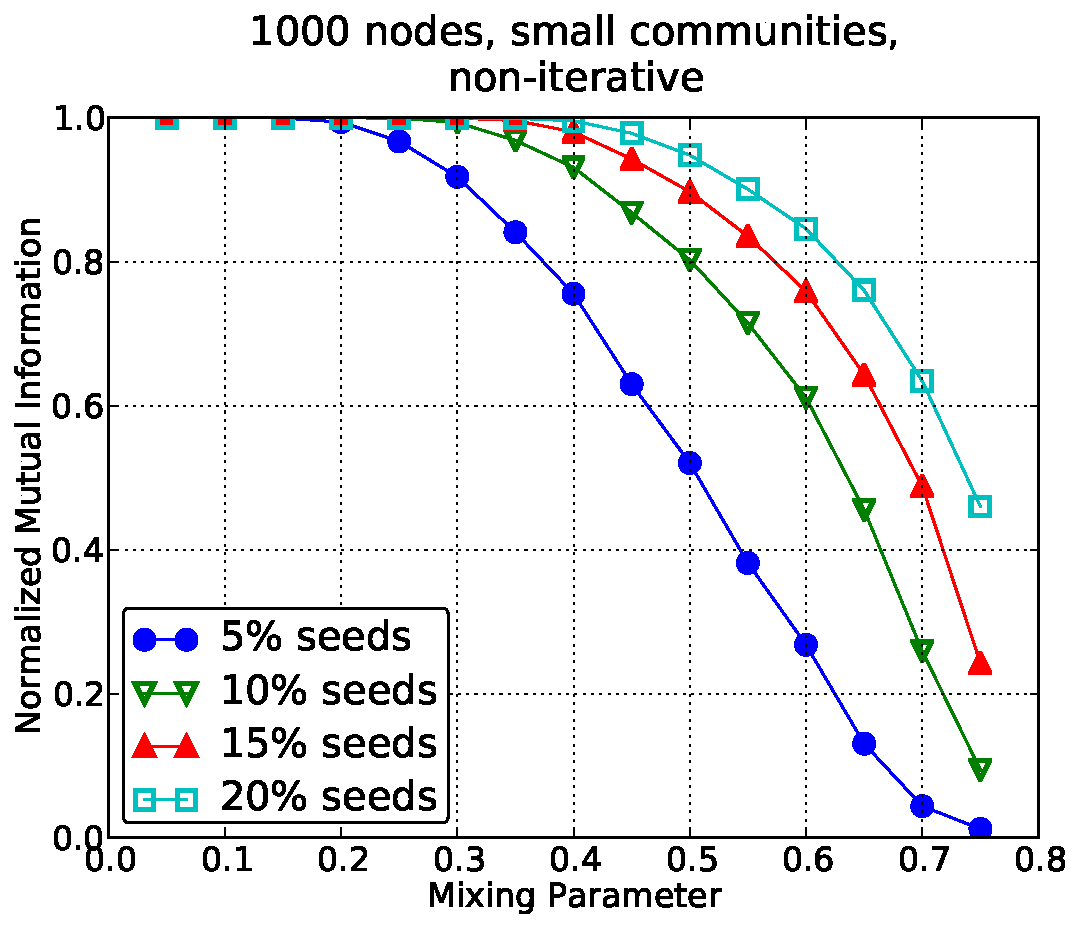
\includegraphics[width=\appplotwidth]{plots/nonoverlap_noniter_a.pdf}
    \end{subfigure}%
    \begin{subfigure}{0.5\textwidth}
    \centering
    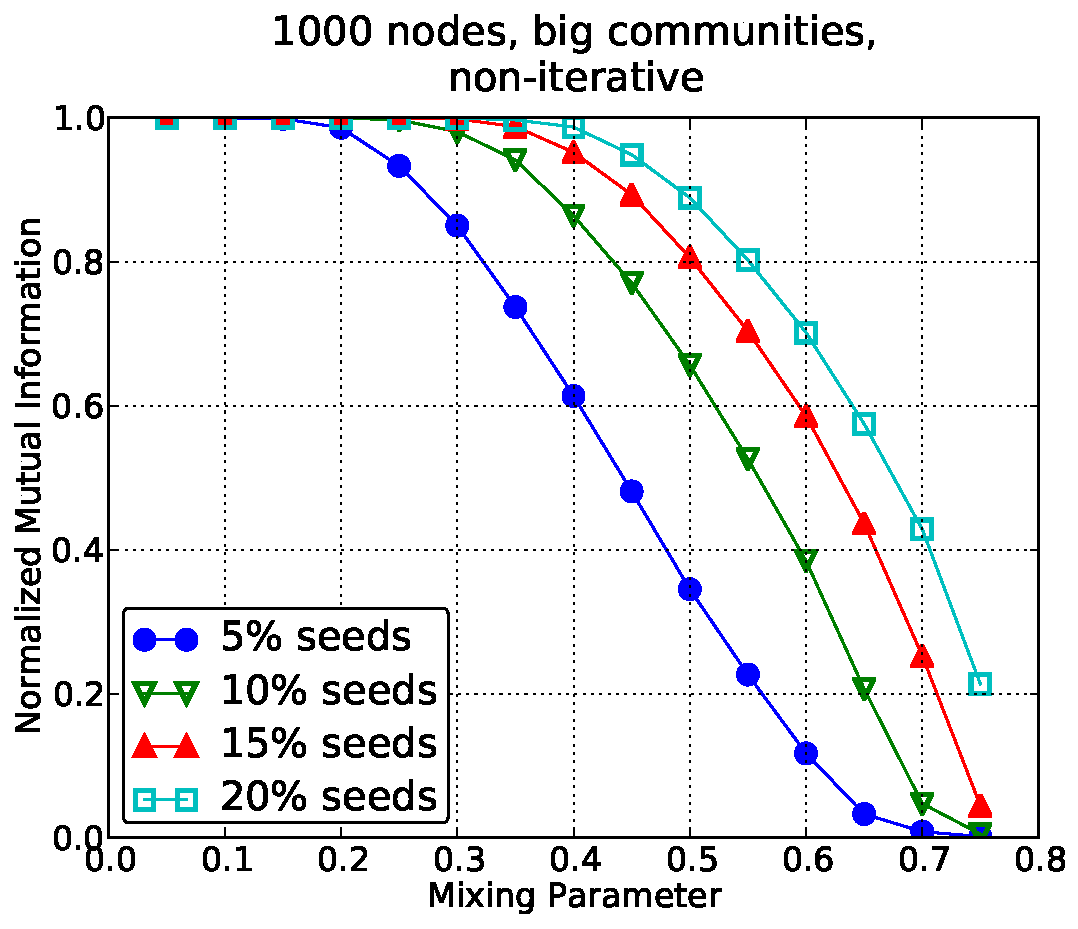
\includegraphics[width=\appplotwidth]{plots/nonoverlap_noniter_b.pdf}
    \end{subfigure}
    \begin{subfigure}{0.5\textwidth}
    \centering
    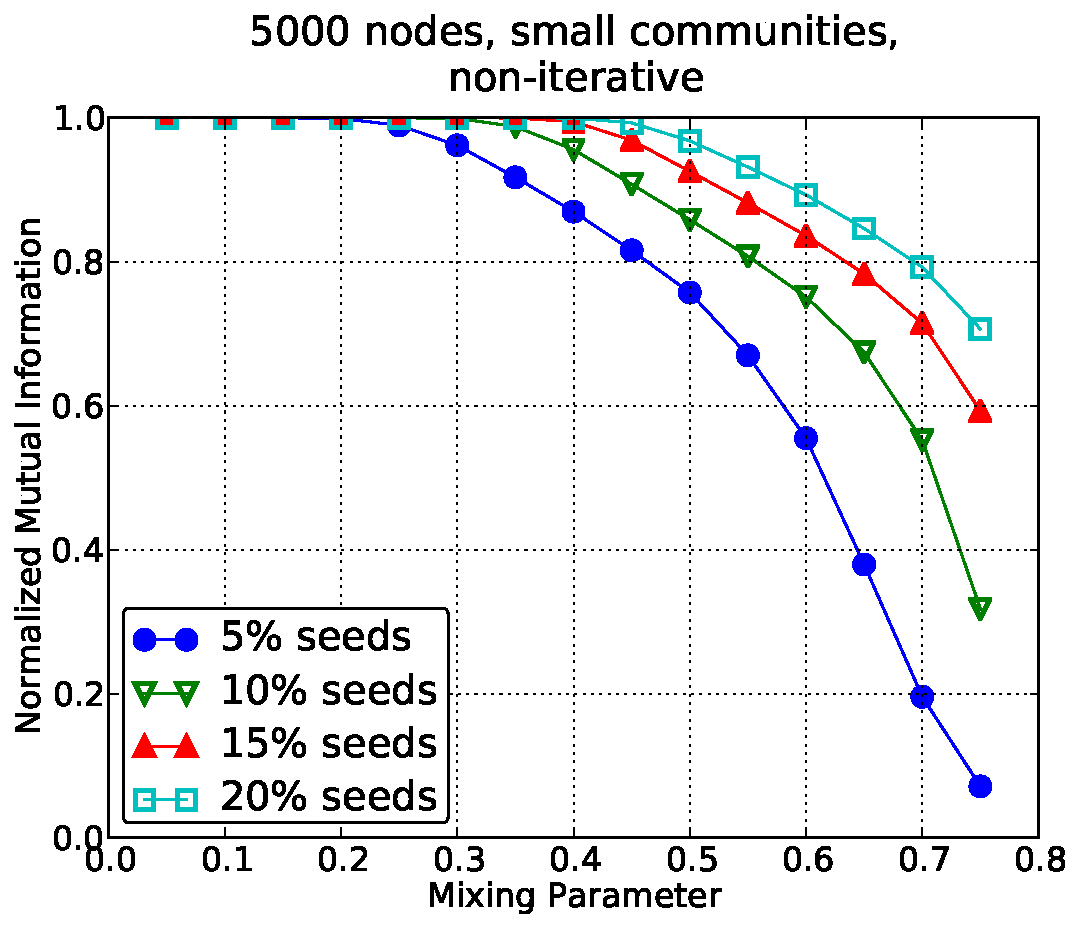
\includegraphics[width=\appplotwidth]{plots/nonoverlap_noniter_c.pdf}
    \end{subfigure}%
    \begin{subfigure}{0.5\textwidth}
    \centering
    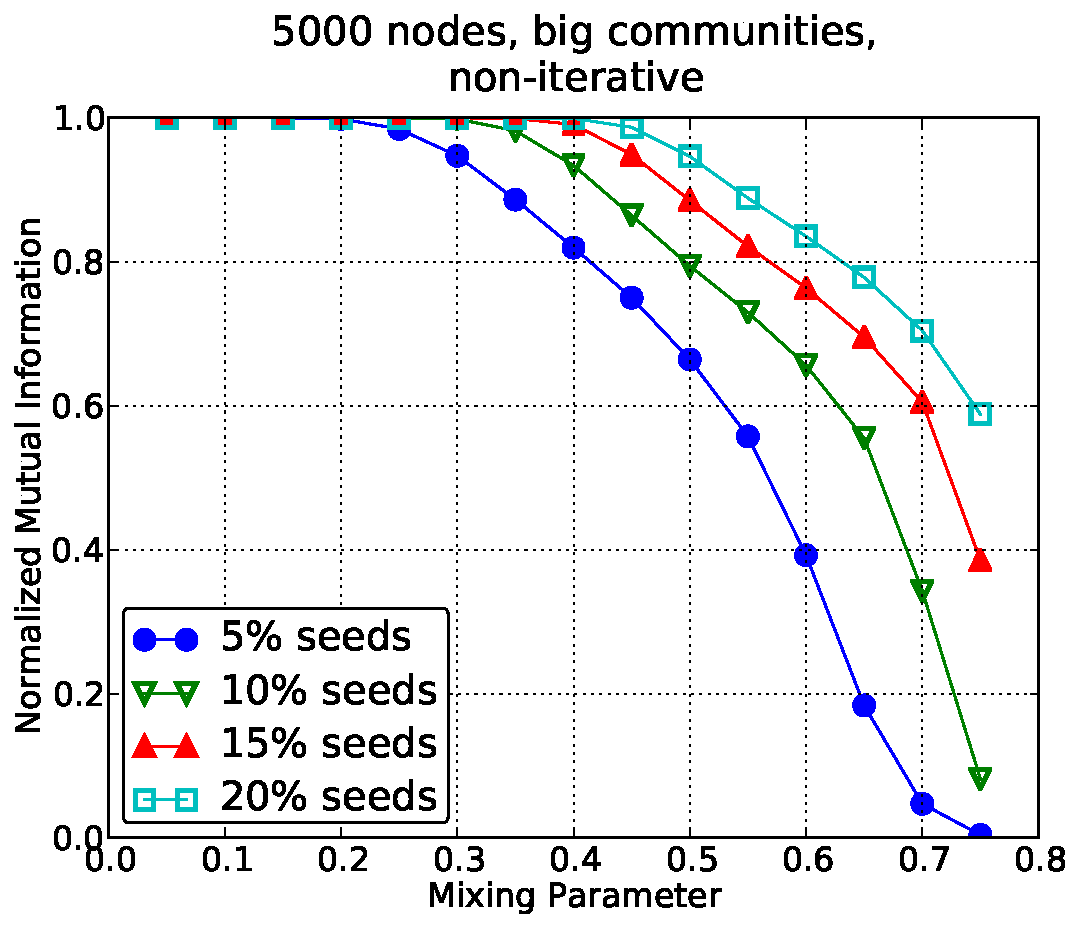
\includegraphics[width=\appplotwidth]{plots/nonoverlap_noniter_d.pdf}
    \end{subfigure}
    \caption{Non-iterative method for non-overlapping communities.}\label{fig:no_iter_no_overlap}
\end{figure}
%
\begin{figure}[h!]
    \centering
    \begin{subfigure}{0.5\textwidth}
    \centering
    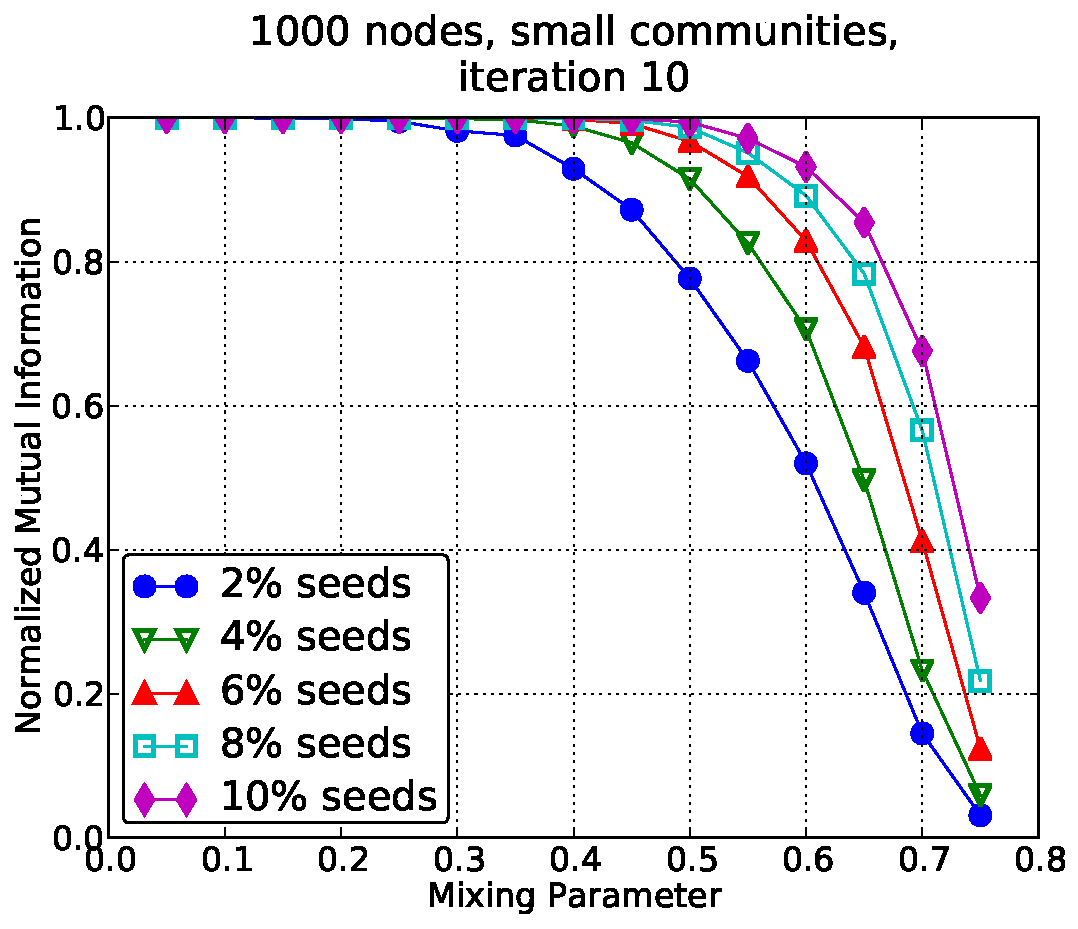
\includegraphics[width=\appplotwidth]{plots/nonoverlap_iter_a.pdf}
    \end{subfigure}%
    \begin{subfigure}{0.5\textwidth}
    \centering
    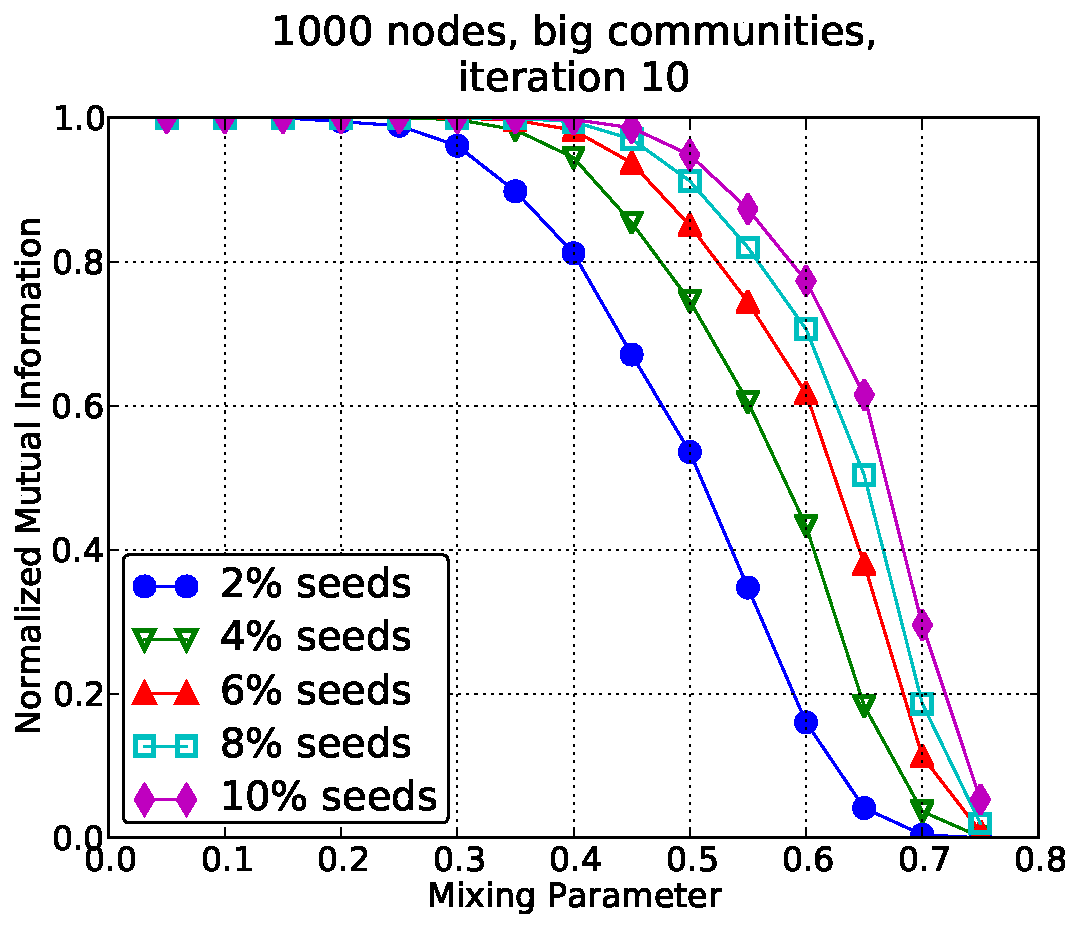
\includegraphics[width=\appplotwidth]{plots/nonoverlap_iter_b.pdf}
    \end{subfigure}
    \begin{subfigure}{0.5\textwidth}
    \centering
    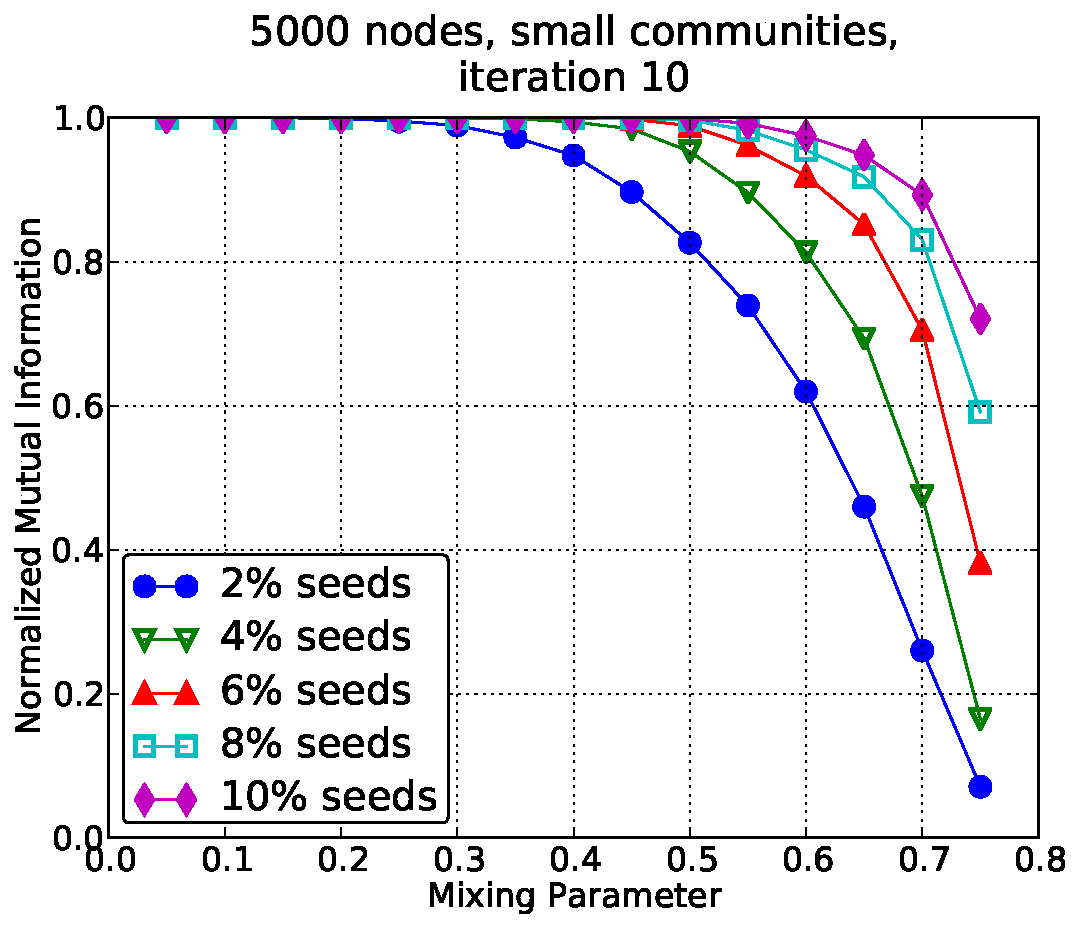
\includegraphics[width=\appplotwidth]{plots/nonoverlap_iter_c.pdf}
    \end{subfigure}%
    \begin{subfigure}{0.5\textwidth}
    \centering
    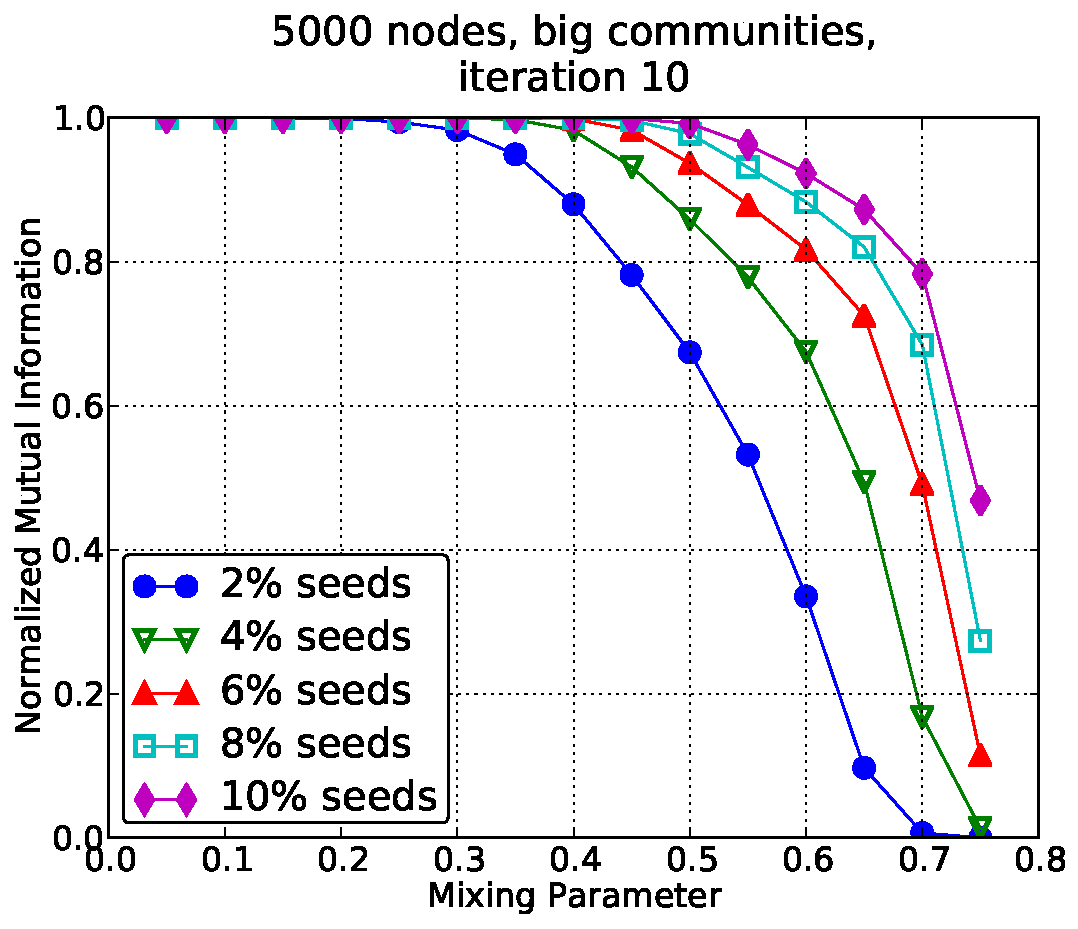
\includegraphics[width=\appplotwidth]{plots/nonoverlap_iter_d.pdf}
    \end{subfigure}
    \caption{Iterative method for non-overlapping communities.}\label{fig:iter_no_overlap}
\end{figure}
%

%\begin{figure}[h!]
%    \centering
%    \begin{subfigure}{0.5\textwidth}
%    \centering
%    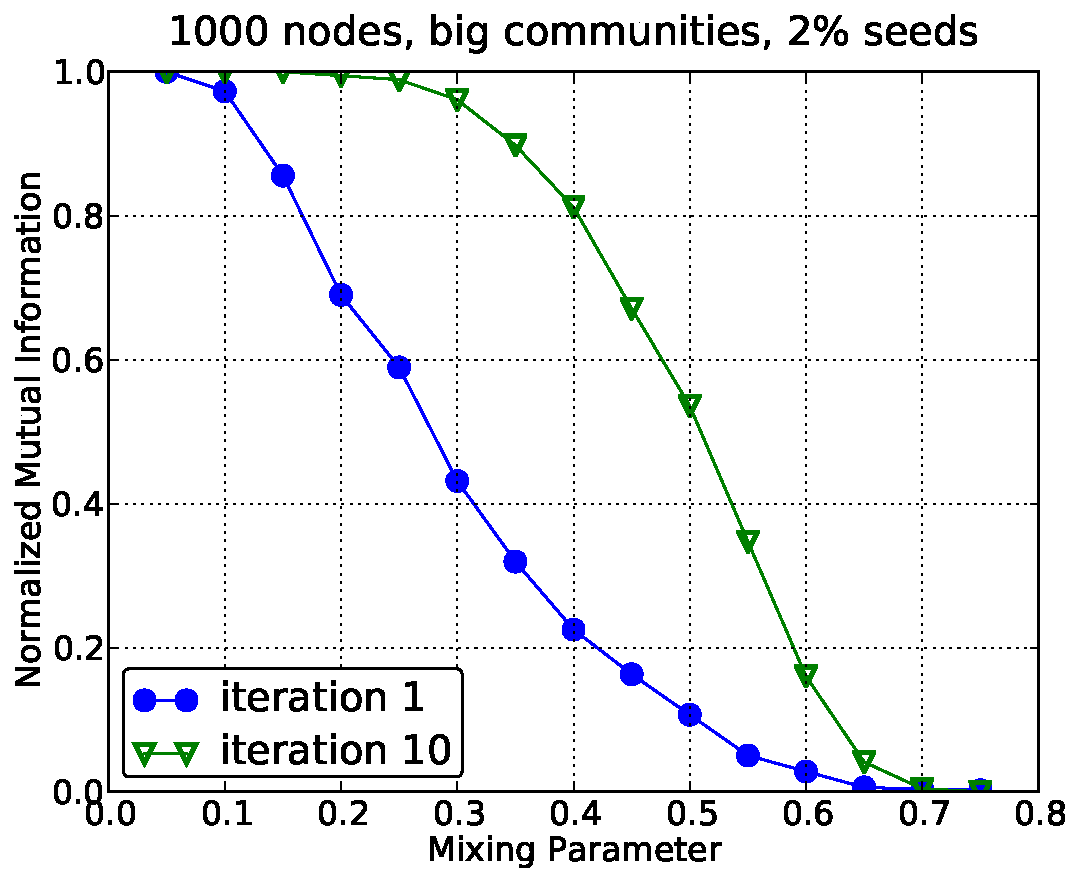
\includegraphics[width=\plotwidth]{plots/nonoverlap_compare_a.pdf}
%    \end{subfigure}%
%    \begin{subfigure}{0.5\textwidth}
%    \centering
%    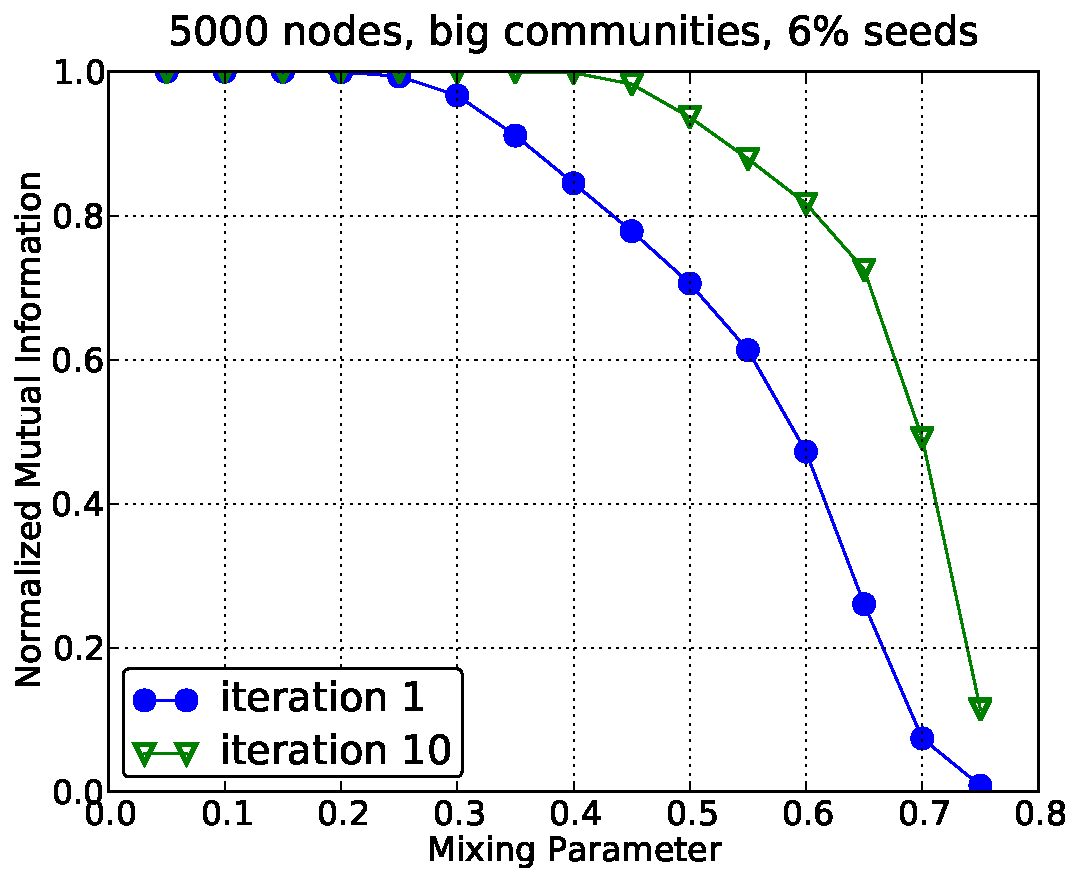
\includegraphics[width=\plotwidth]{plots/nonoverlap_compare_b.pdf}
%    \end{subfigure}
%    \caption{Comparison between the iterative and non-iterative method for 
%		non-overlapping communities.}\label{fig:compare_iter_no_overlap}
%\end{figure}

\begin{figure}[h!]
    \centering
    \begin{subfigure}{0.35\textwidth}
    \centering
    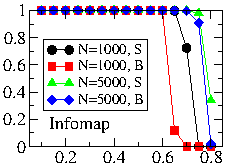
\includegraphics[width=\otherplotswidth]{lfrpaper/1_split_kropped.pdf}
    \end{subfigure}%
    \begin{subfigure}{0.35\textwidth}
    \centering
    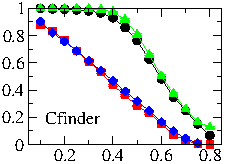
\includegraphics[width=\otherplotswidth]{lfrpaper/2_split_kropped.pdf}
    \end{subfigure}%
    \begin{subfigure}{0.35\textwidth}
    \centering
    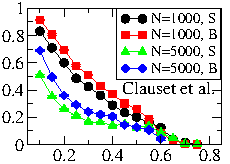
\includegraphics[width=\otherplotswidth]{lfrpaper/3_split_kropped.pdf}
    \end{subfigure}
    \begin{subfigure}{0.35\textwidth}
    \centering
    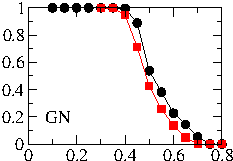
\includegraphics[width=\otherplotswidth]{lfrpaper/4_split_kropped.pdf}
    \end{subfigure}%
    \begin{subfigure}{0.35\textwidth}
    \centering
    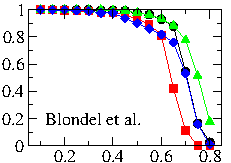
\includegraphics[width=\otherplotswidth]{lfrpaper/5_split_kropped.pdf}
    \end{subfigure}%
    \begin{subfigure}{0.35\textwidth}
    \centering
    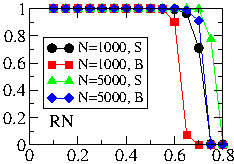
\includegraphics[width=\otherplotswidth]{lfrpaper/6_split_kropped.pdf}
    \end{subfigure}%
    \caption{
        Plots for Infomap, CFinder, the algorithm of Clauset \etal, Girvan-Newman (GN), Blondel \etal, 
        and the Pott's model approach by Ronhovde and Nussinov (RN) on the LFR benchmark for non-overlapping 
		communities. As usual, the NMI-value ($y$-axis) is plotted against the mixing factor ($x$-axis).
        Tests were performed on graphs with 1000 and 5000 nodes with big (B) and small (S) communities.
        Reproduced from~\cite{LF09}.
    }\label{fig:Infomap_etal}
\end{figure}

\begin{figure}[h!]
    \centering
    \begin{subfigure}{0.5\textwidth}
    \centering
    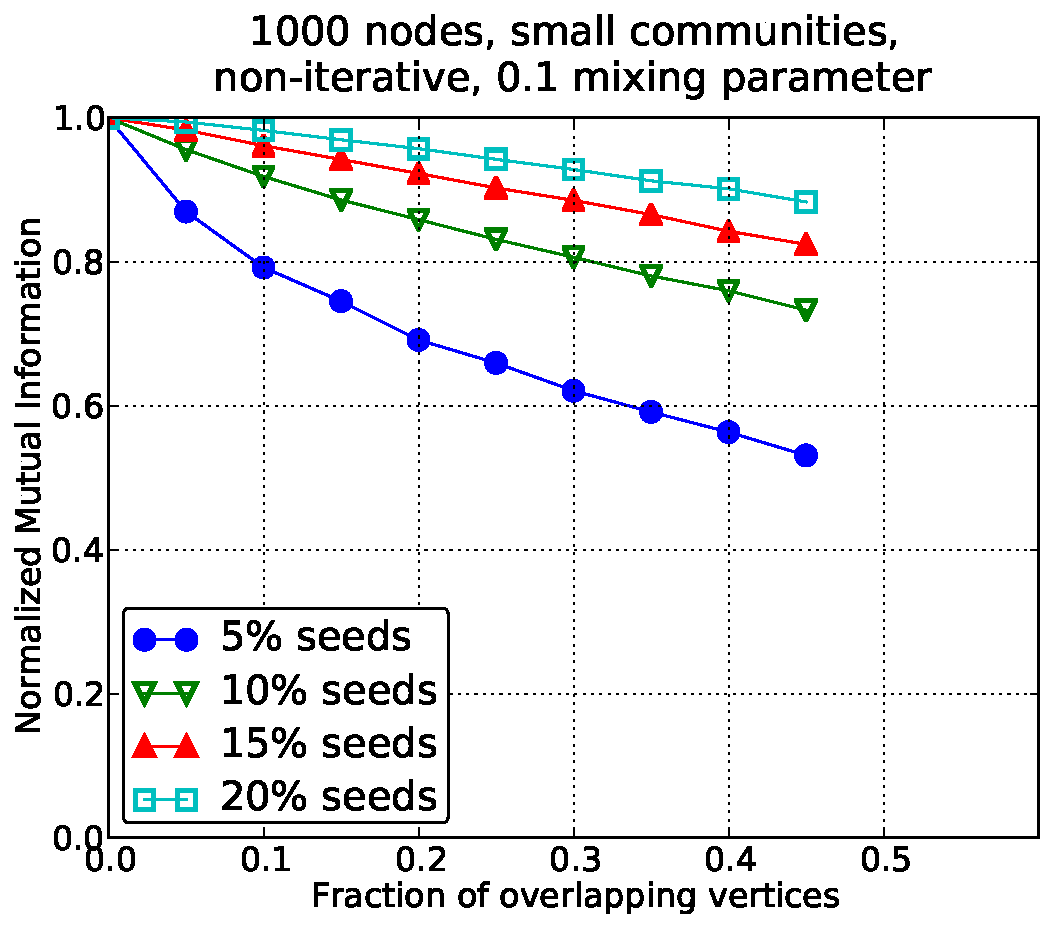
\includegraphics[width=\appplotwidth]{plots/overlap_noniter_1mu_a.pdf}
    \end{subfigure}%
    \begin{subfigure}{0.5\textwidth}
    \centering
    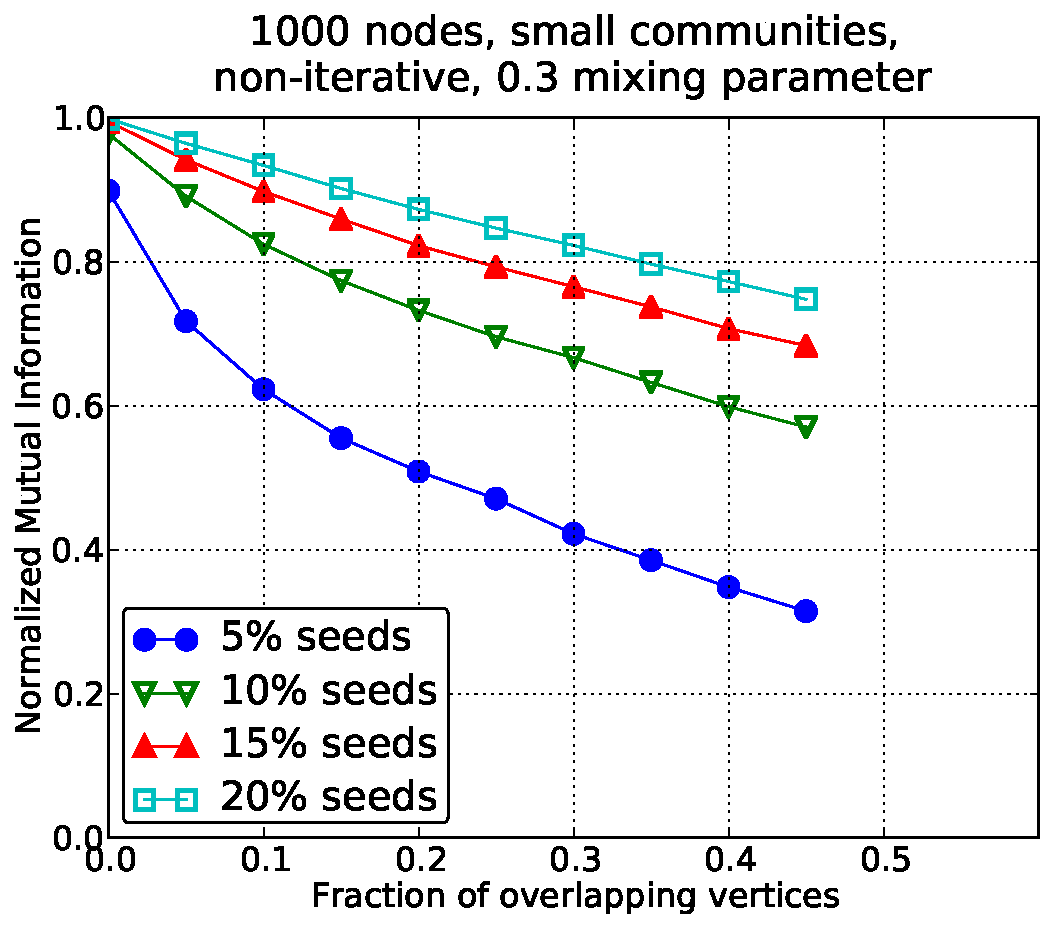
\includegraphics[width=\appplotwidth]{plots/overlap_noniter_3mu_a.pdf}
    \end{subfigure}
    \begin{subfigure}{0.5\textwidth}
    \centering
    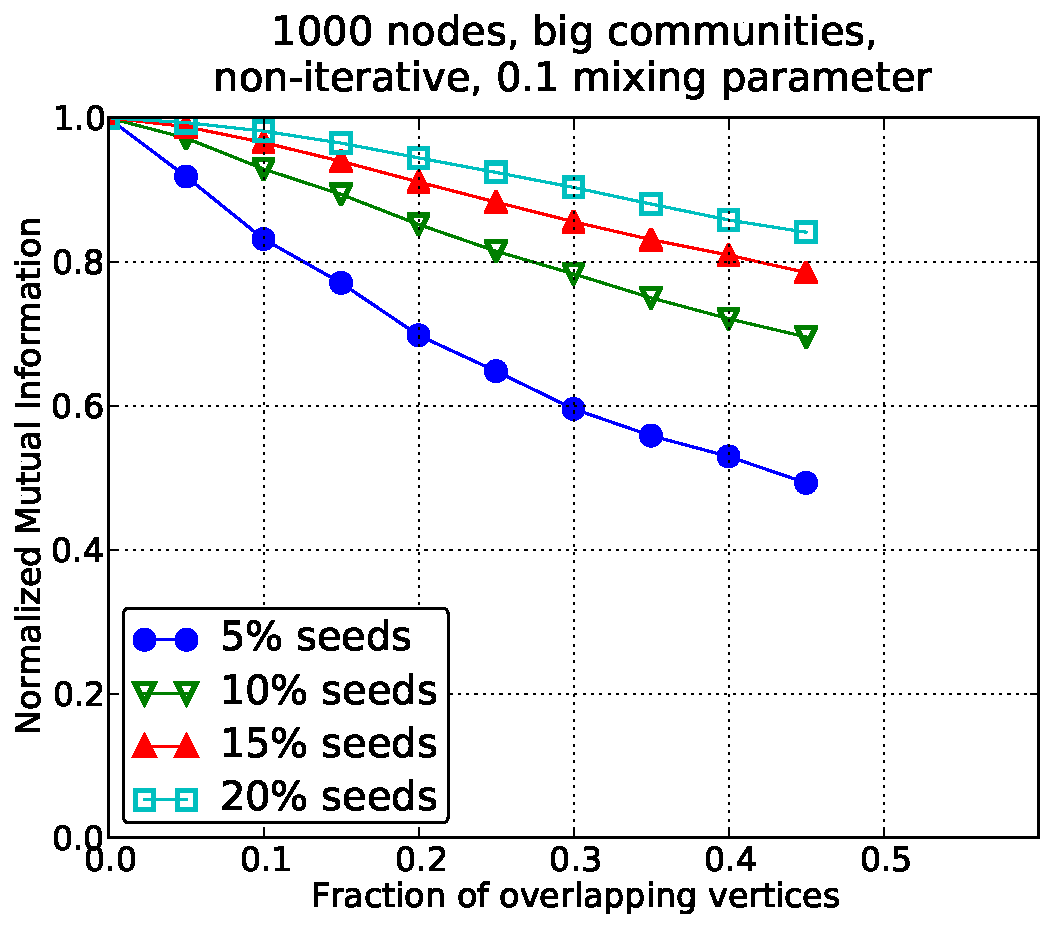
\includegraphics[width=\appplotwidth]{plots/overlap_noniter_1mu_b.pdf}
    \end{subfigure}%
    \begin{subfigure}{0.5\textwidth}
    \centering
    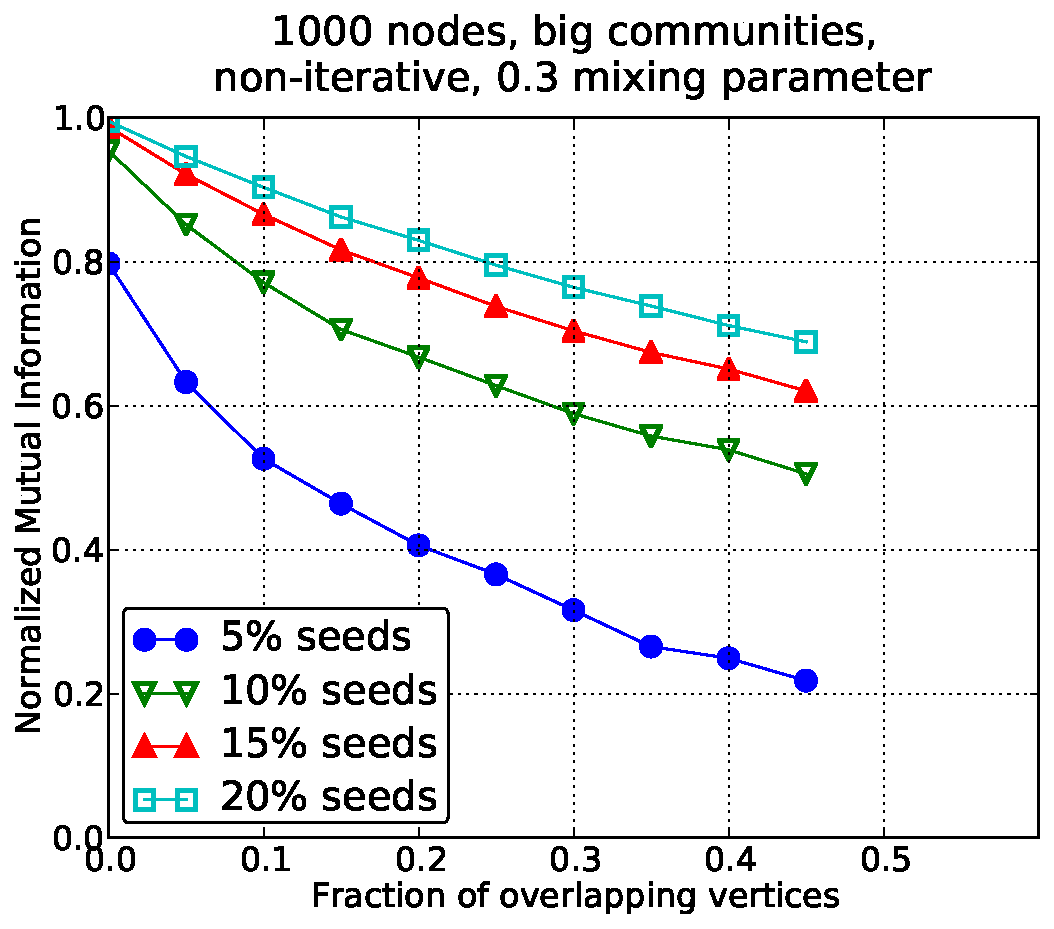
\includegraphics[width=\appplotwidth]{plots/overlap_noniter_3mu_b.pdf}
    \end{subfigure}
    \caption{Non-iterative method for overlapping communities on 1000 nodes.}\label{fig:no_iter_overlap_1000N}
\end{figure}
%
\begin{figure}[h!]
    \centering
    \begin{subfigure}{0.5\textwidth}
    \centering
    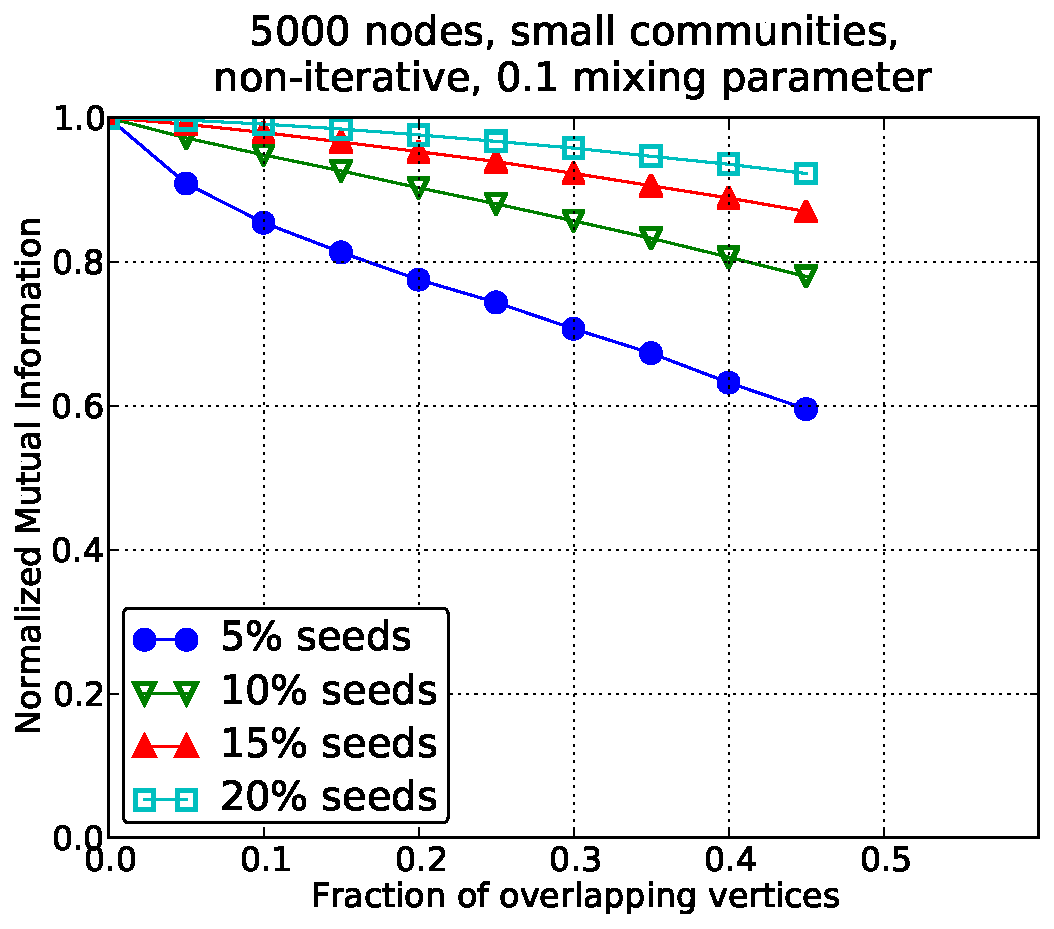
\includegraphics[width=\appplotwidth]{plots/overlap_noniter_1mu_c.pdf}
    \end{subfigure}%
    \begin{subfigure}{0.5\textwidth}
    \centering
    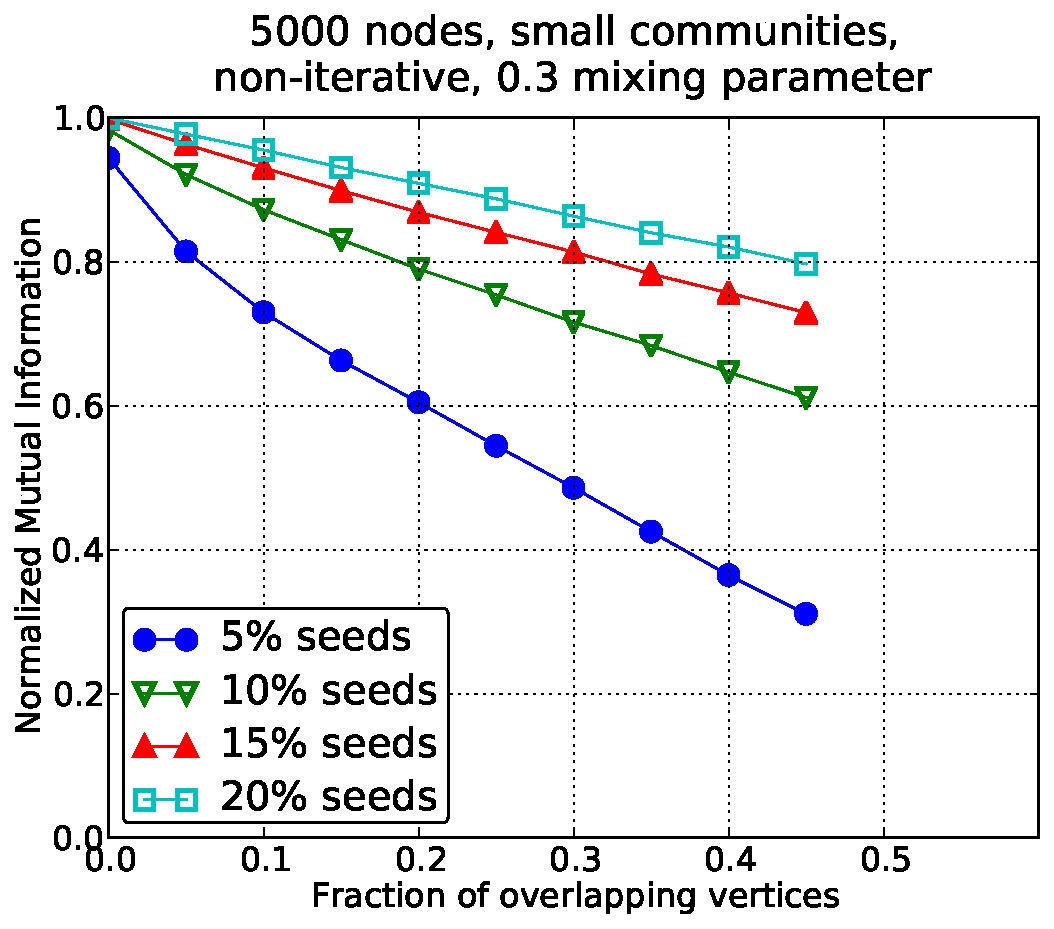
\includegraphics[width=\appplotwidth]{plots/overlap_noniter_3mu_c.pdf}
    \end{subfigure}
    \begin{subfigure}{0.5\textwidth}
    \centering
    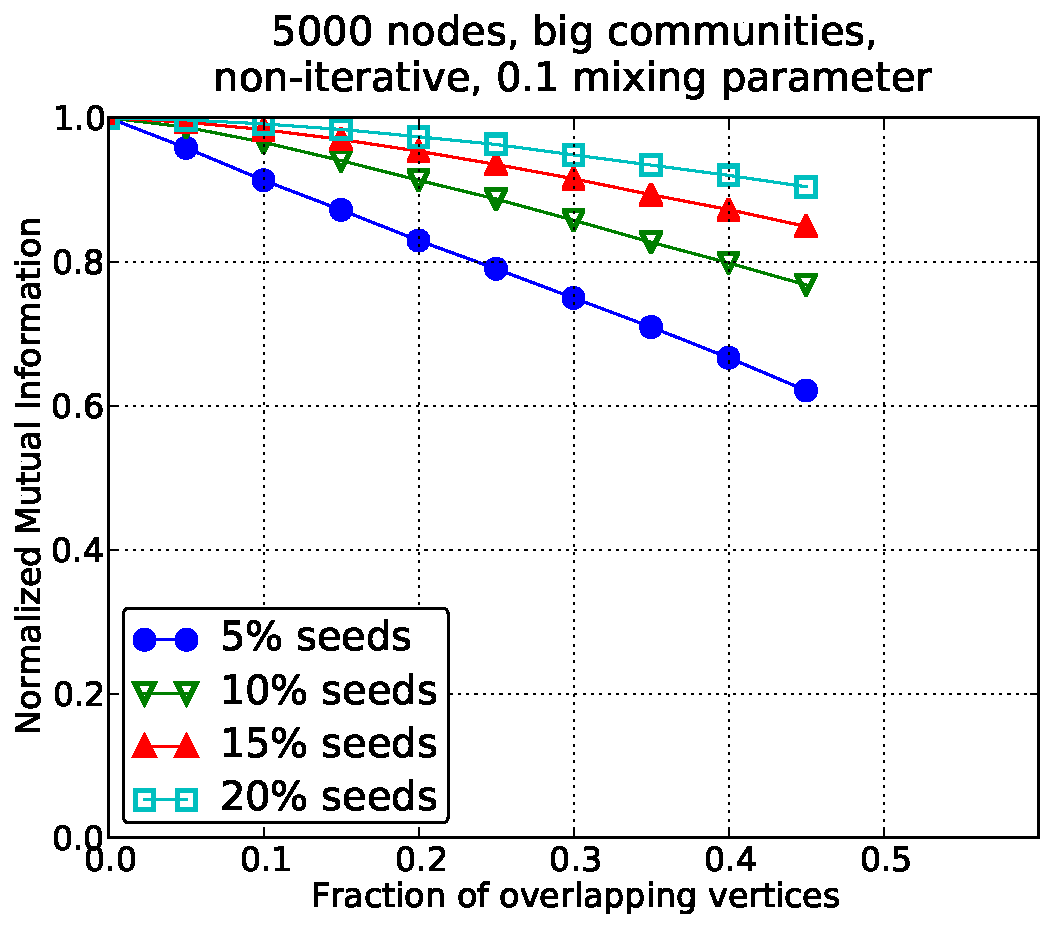
\includegraphics[width=\appplotwidth]{plots/overlap_noniter_1mu_d.pdf}
    \end{subfigure}%
    \begin{subfigure}{0.5\textwidth}
    \centering
    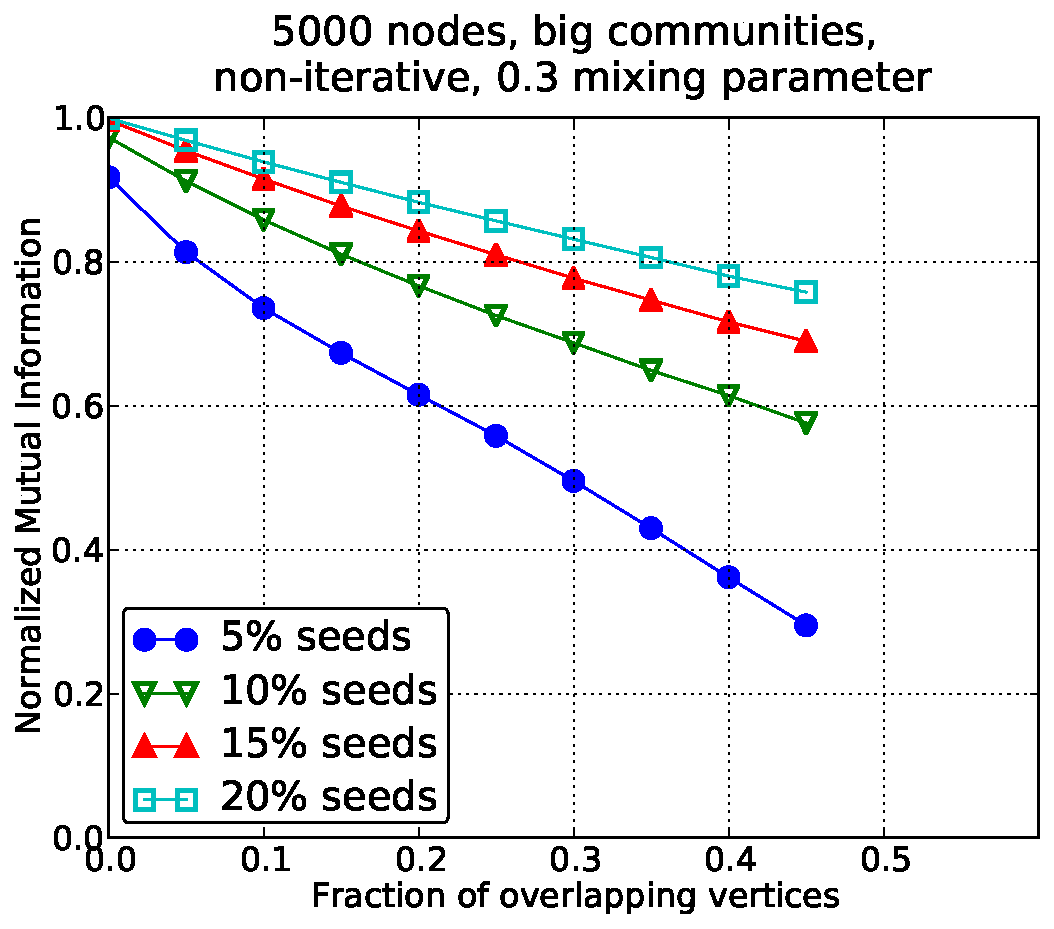
\includegraphics[width=\appplotwidth]{plots/overlap_noniter_3mu_d.pdf}
    \end{subfigure}
    \caption{Non-iterative method for overlapping communities on 5000 nodes.}\label{fig:no_iter_overlap_5000N}
\end{figure}
%
\begin{figure}[h!]
    \centering
    \begin{subfigure}{0.5\textwidth}
    \centering
    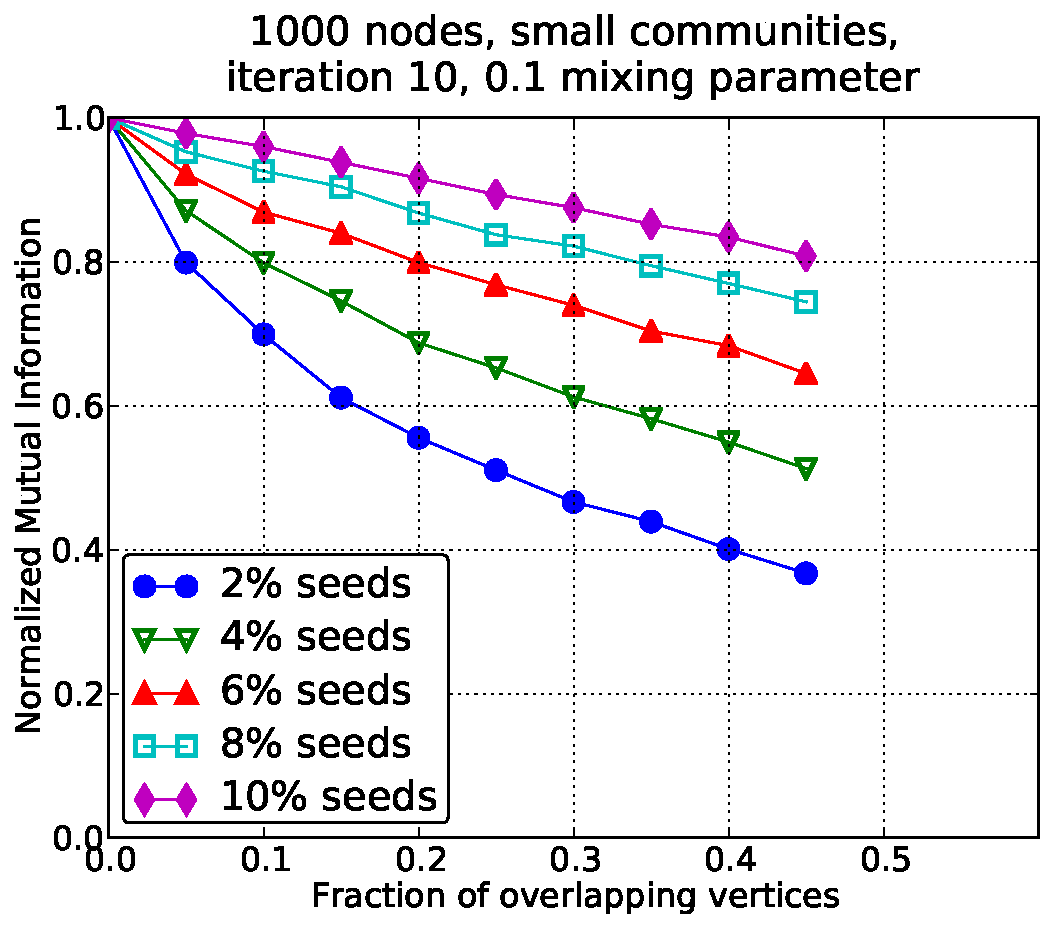
\includegraphics[width=\appplotwidth]{plots/overlap_iter_1mu_a.pdf}
    \end{subfigure}%
    \begin{subfigure}{0.5\textwidth}
    \centering
    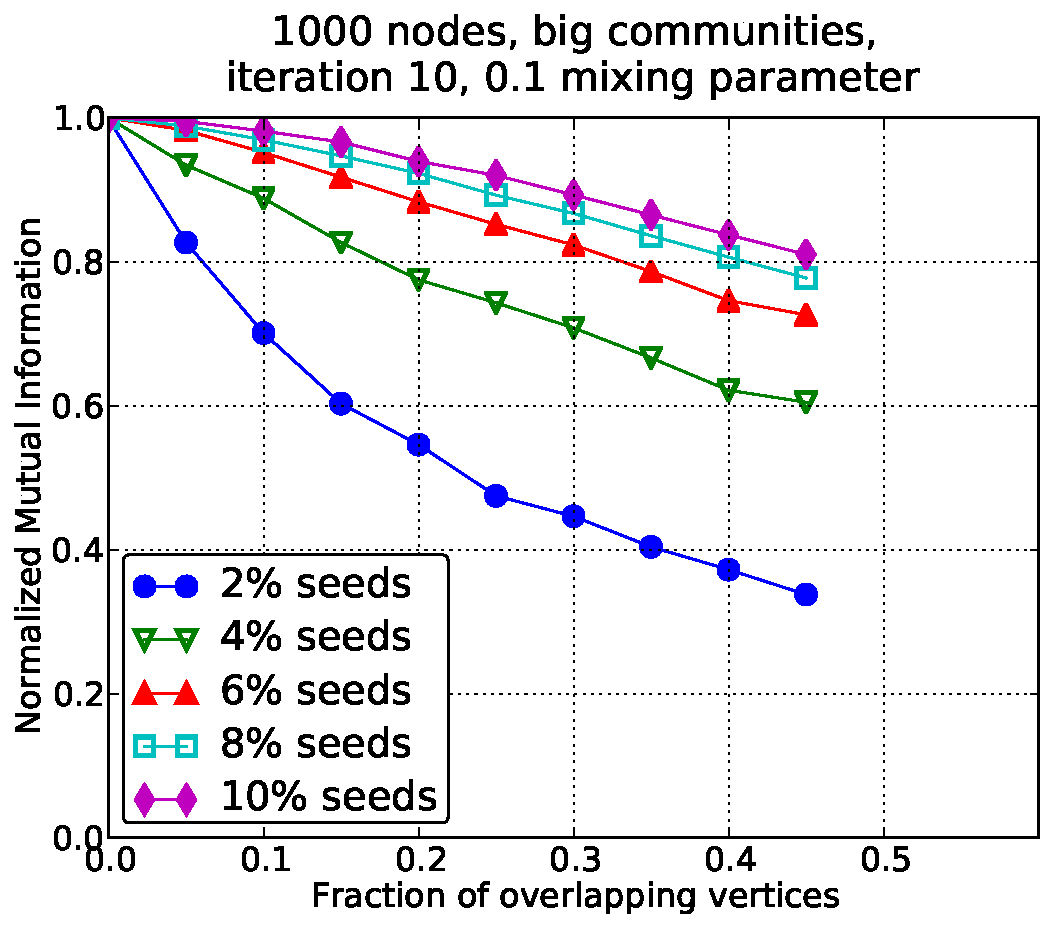
\includegraphics[width=\appplotwidth]{plots/overlap_iter_1mu_b.pdf}
    \end{subfigure}
    \begin{subfigure}{0.5\textwidth}
    \centering
    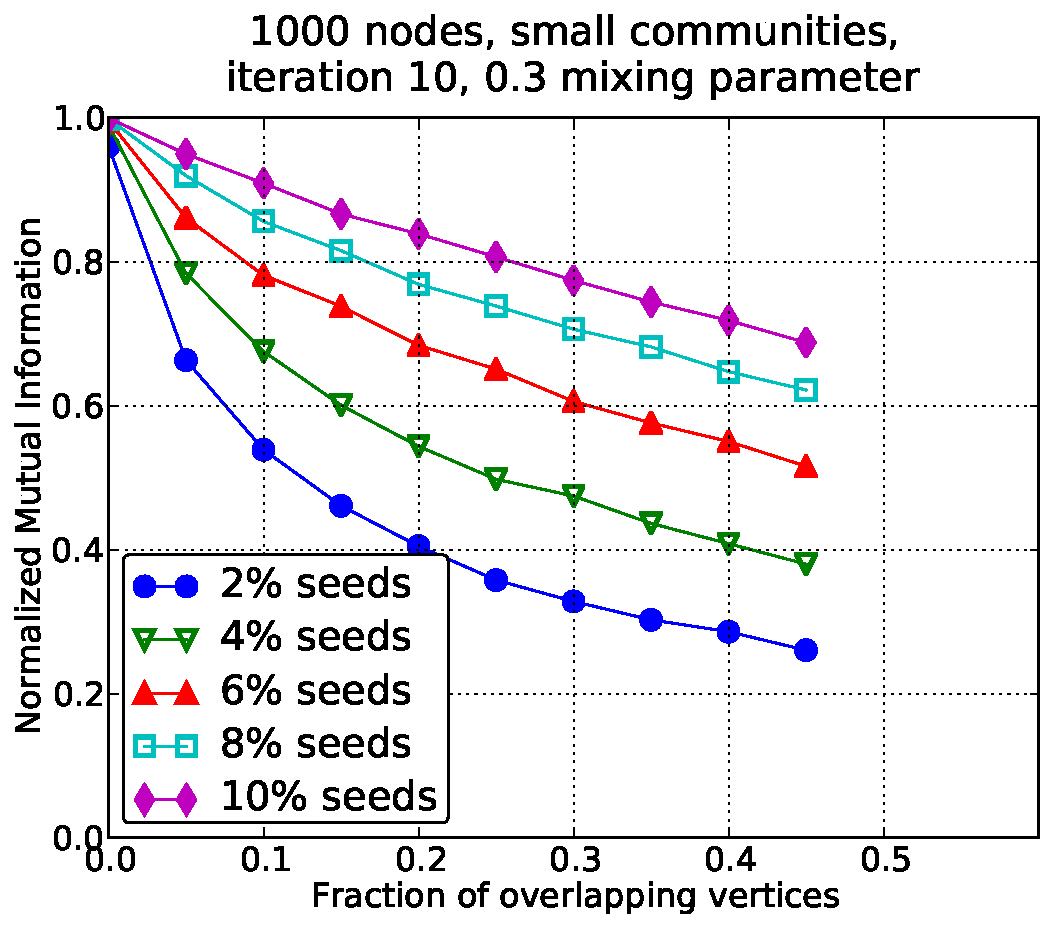
\includegraphics[width=\appplotwidth]{plots/overlap_iter_3mu_a.pdf}
    \end{subfigure}%
    \begin{subfigure}{0.5\textwidth}
    \centering
    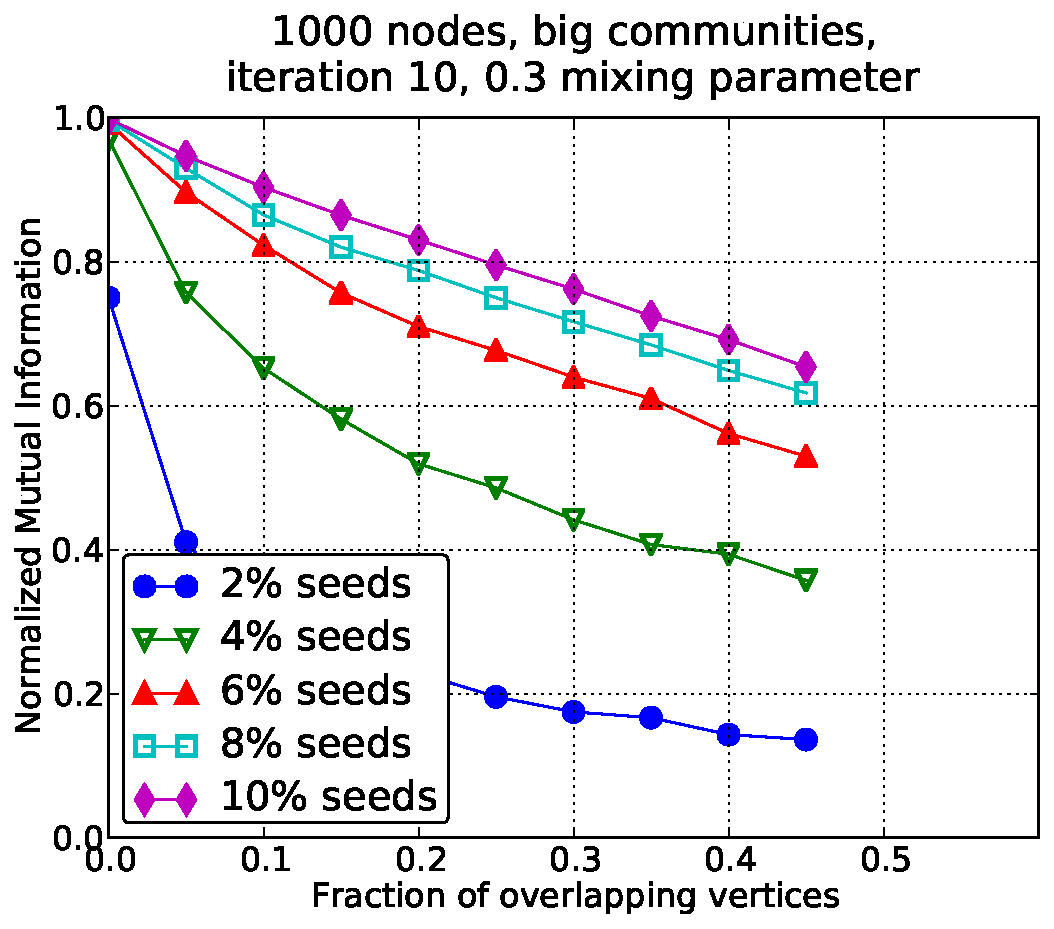
\includegraphics[width=\appplotwidth]{plots/overlap_iter_3mu_b.pdf}
    \end{subfigure}
    \caption{Iterative method for overlapping communities on 1000 nodes.}\label{fig:iter_overlap_1000N}
\end{figure}
%
\begin{figure}[h!]
    \centering
    \begin{subfigure}{0.5\textwidth}
    \centering
    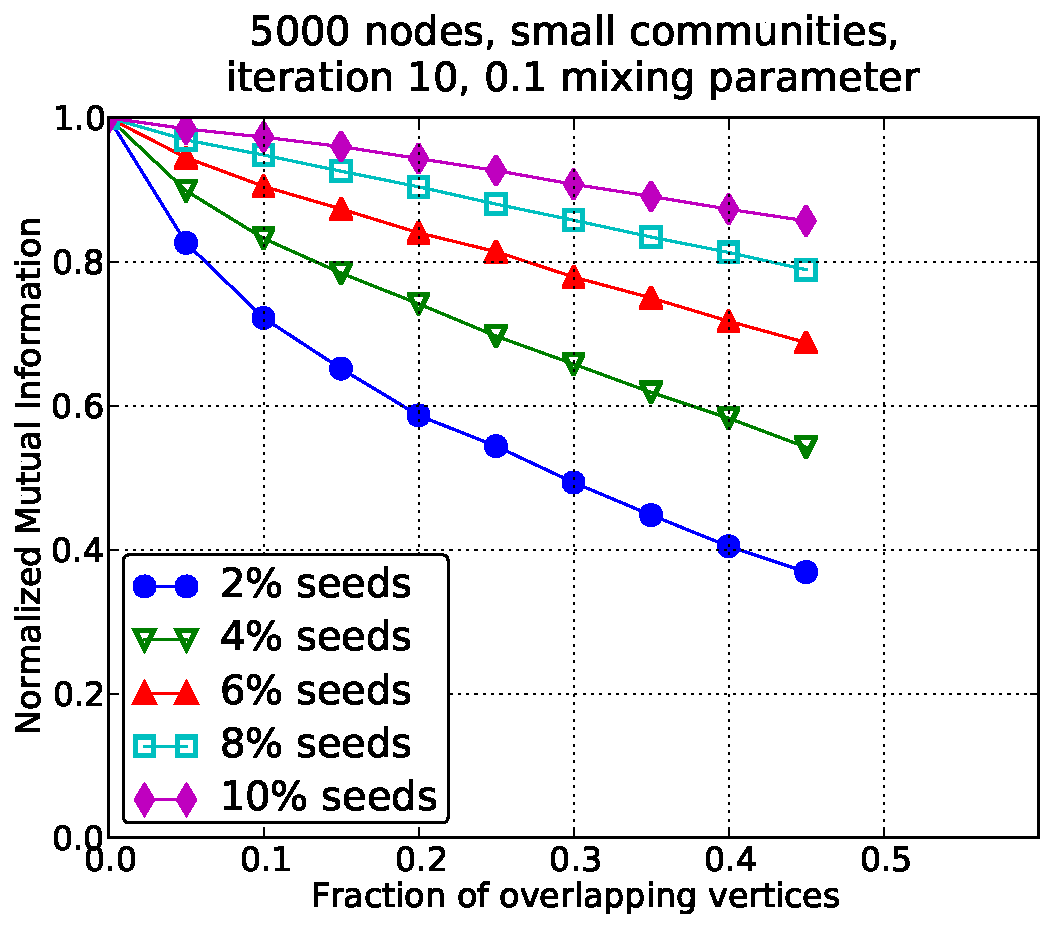
\includegraphics[width=\appplotwidth]{plots/overlap_iter_1mu_c.pdf}
    \end{subfigure}%
    \begin{subfigure}{0.5\textwidth}
    \centering
    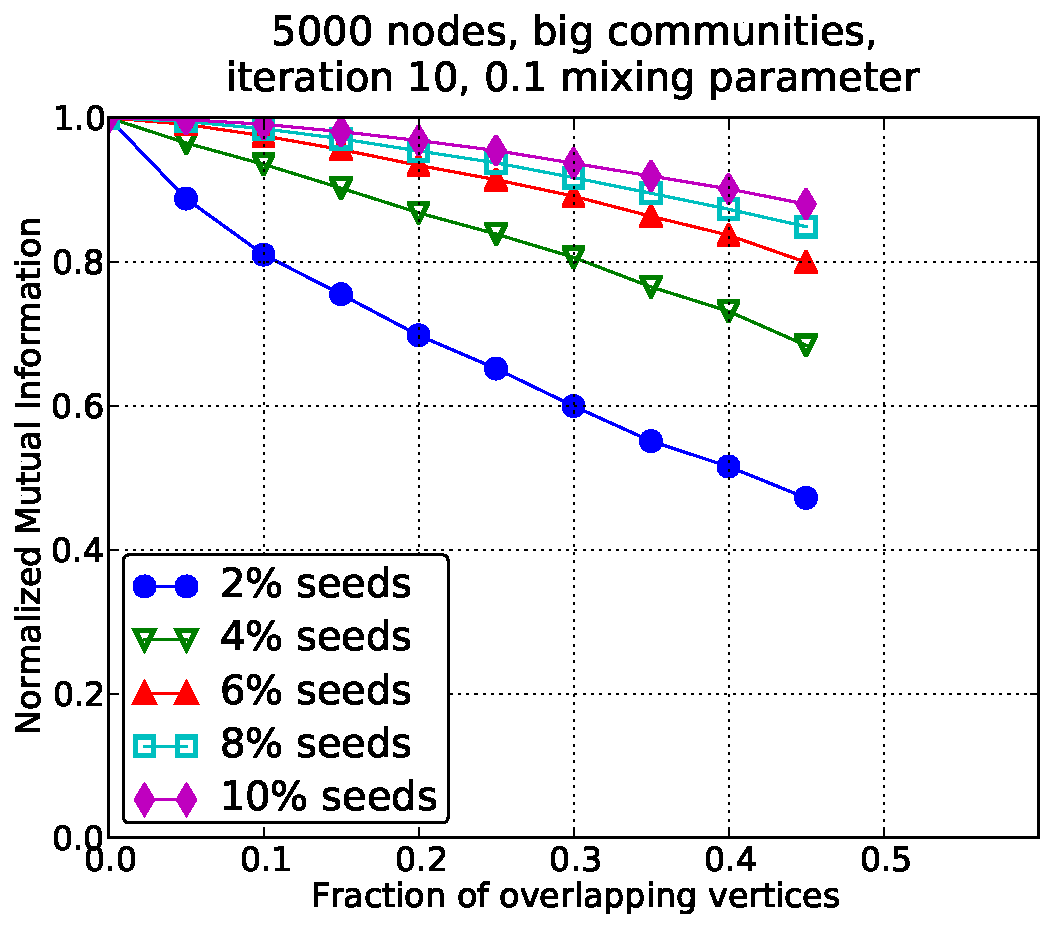
\includegraphics[width=\appplotwidth]{plots/overlap_iter_1mu_d.pdf}
    \end{subfigure}
    \begin{subfigure}{0.5\textwidth}
    \centering
    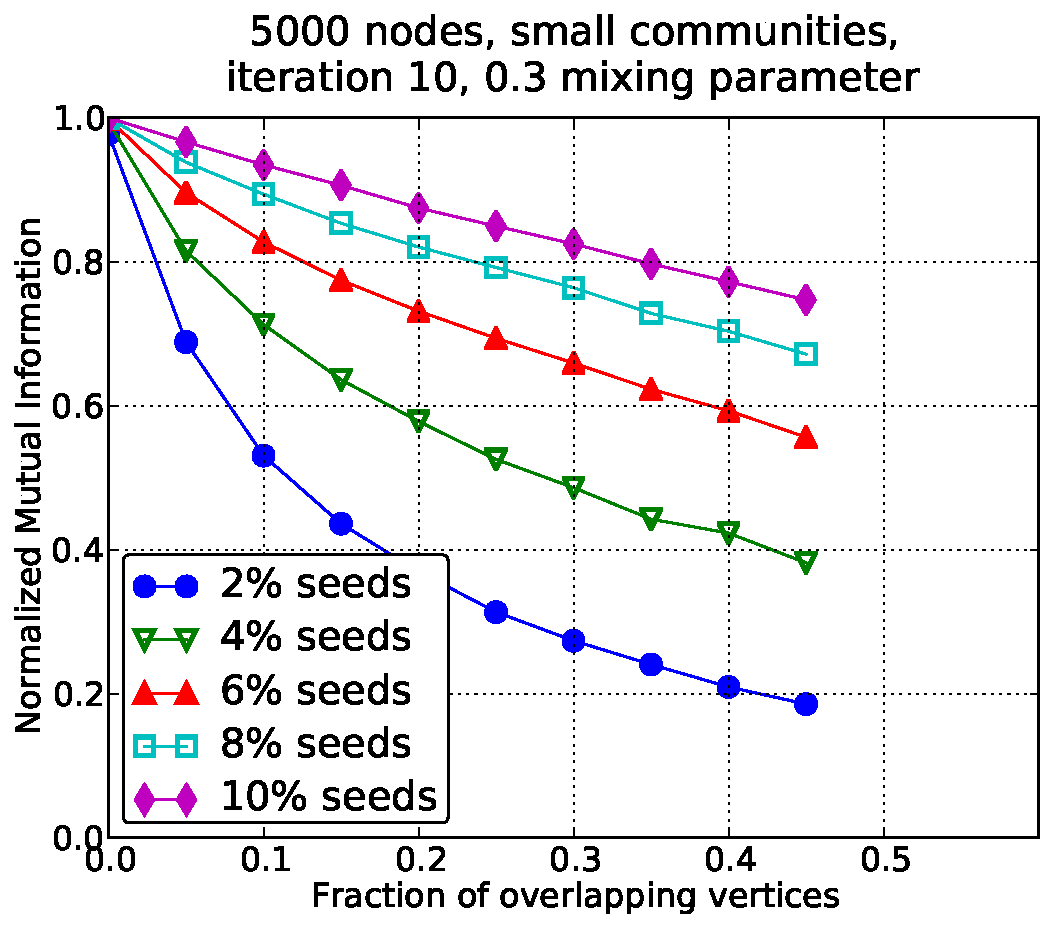
\includegraphics[width=\appplotwidth]{plots/overlap_iter_3mu_c.pdf}
    \end{subfigure}%
    \begin{subfigure}{0.5\textwidth}
    \centering
    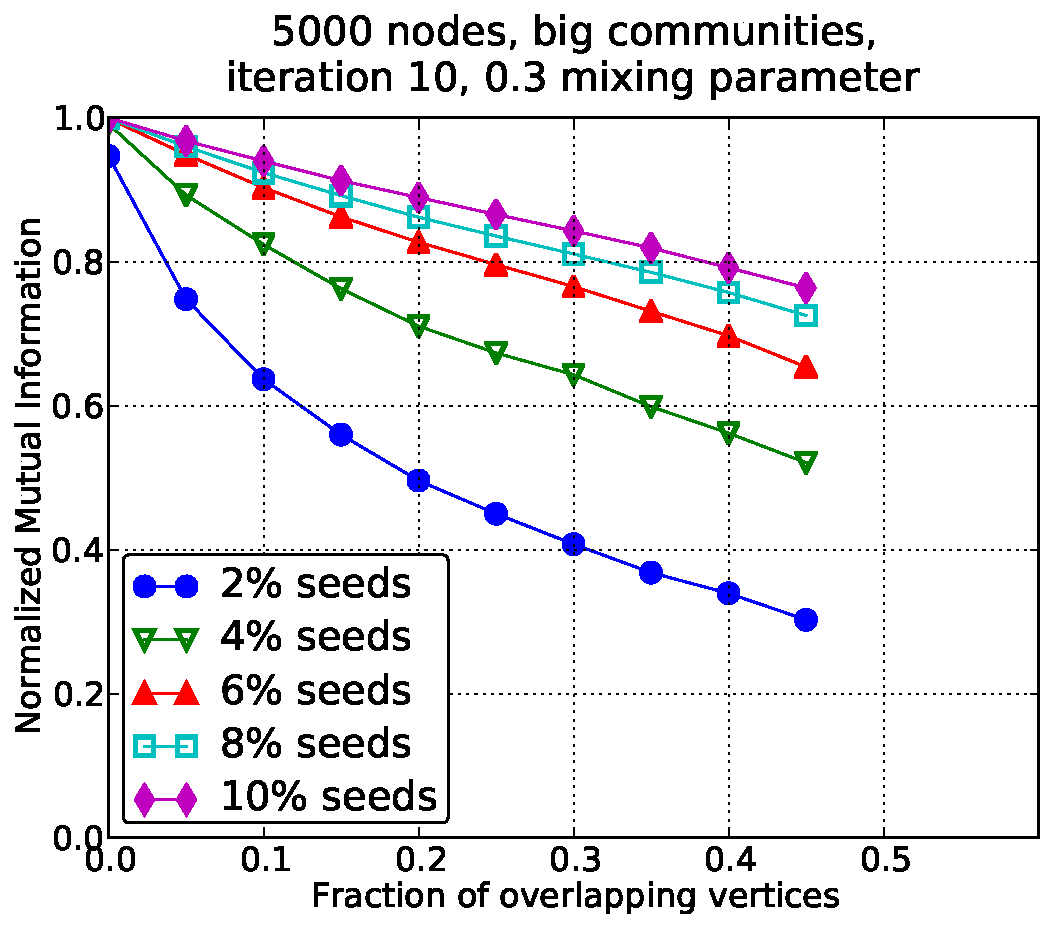
\includegraphics[width=\appplotwidth]{plots/overlap_iter_3mu_d.pdf}
    \end{subfigure}
    \caption{Iterative method for overlapping communities on 5000 nodes.}\label{fig:iter_overlap_5000N}
\end{figure}
%
%\begin{figure}[h!]
%    \centering
%    \begin{subfigure}{0.5\textwidth}
%    \centering
%    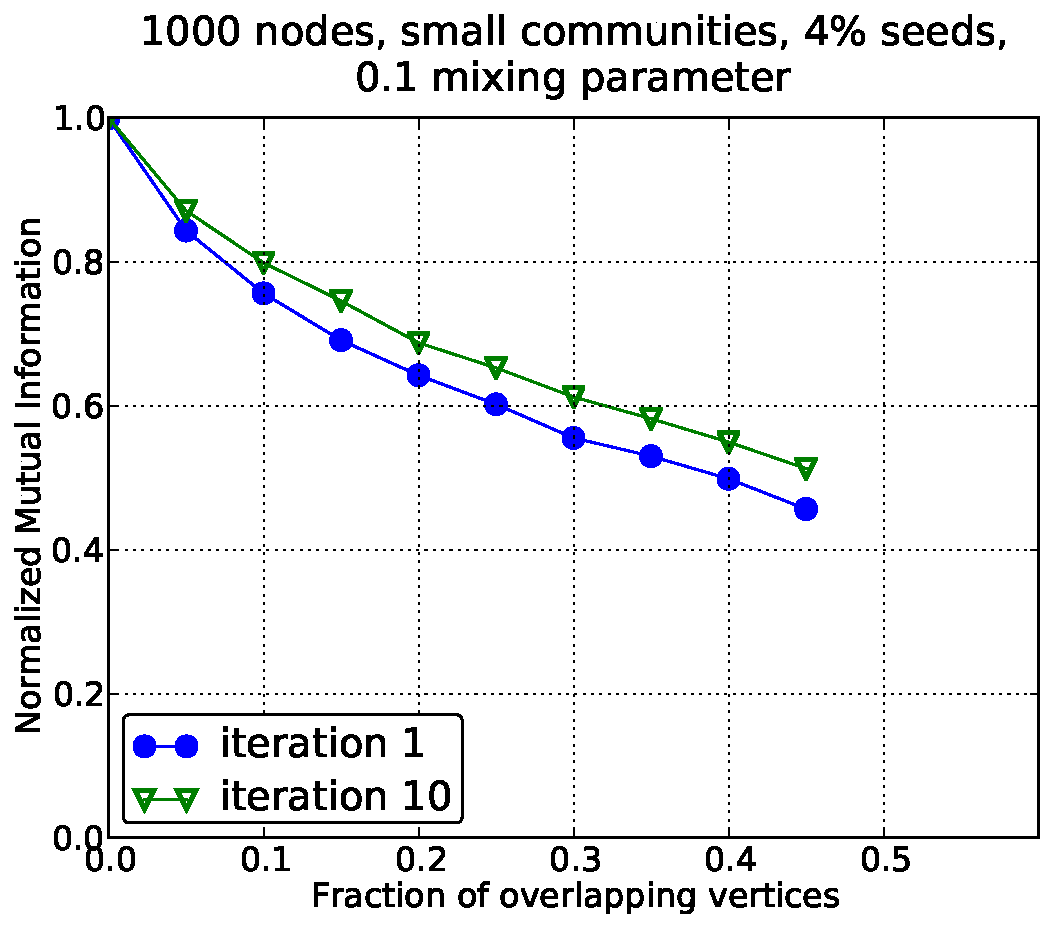
\includegraphics[width=\plotwidth]{plots/overlap_compare_a.pdf}
%    \end{subfigure}%
%    \begin{subfigure}{0.5\textwidth}
%    \centering
%    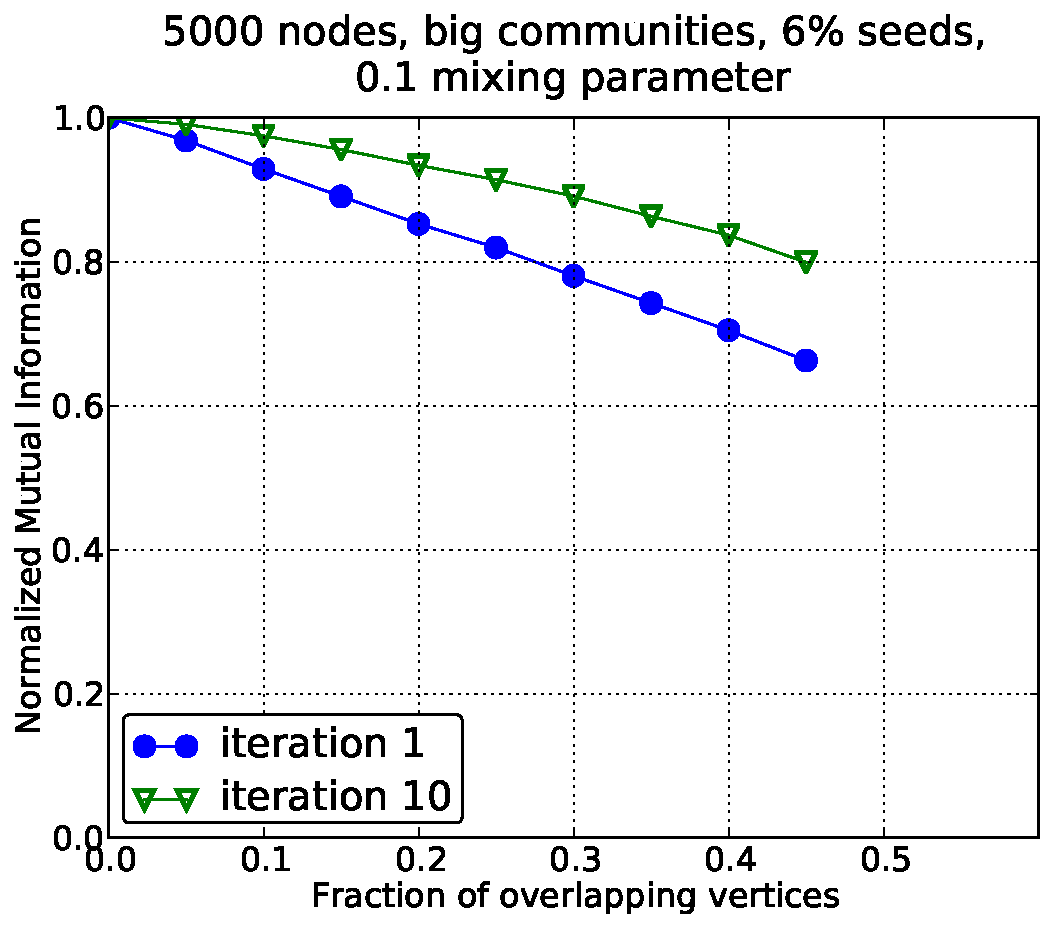
\includegraphics[width=\plotwidth]{plots/overlap_compare_b.pdf}
%    \end{subfigure}
%    \caption{Comparison between the iterative and non-iterative method for overlapping communities.}\label{fig:compare_iter_overlap}
%\end{figure}
%
\begin{figure}[h!]
    \centering
    \begin{subfigure}{0.5\textwidth}
    \centering
    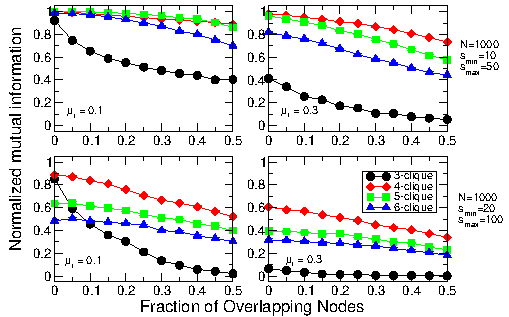
\includegraphics[width=\cfinderwidth]{lfrpaper/fig6.pdf}
    \end{subfigure}%
    \begin{subfigure}{0.5\textwidth}
    \centering
    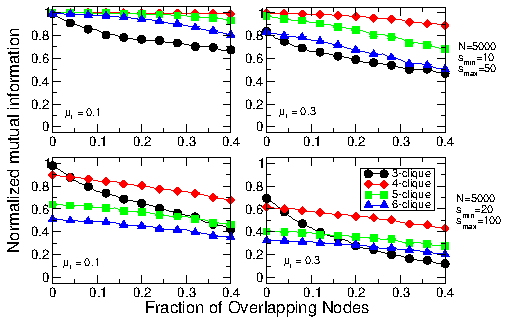
\includegraphics[width=\cfinderwidth]{lfrpaper/fig7.pdf}
    \end{subfigure}%
    \caption{
        Plots for CFinder on the LFR benchmark on graphs with 1000 and 5000 nodes 
		with overlapping communities. Reproduced from~\cite{LF09}.
    }\label{fig:CFinder_overlapping}
\end{figure}



\subsection{Overlapping communities}
Figures~\ref{fig:no_iter_overlap_1000N} and~\ref{fig:no_iter_overlap_5000N} 
show our results for the overlapping case. In the study of Lancichinetti and Fortunato~\cite{LF09}, 
only one algorithm (\emph{Cfinder}~\cite{PDFV05}) for overlapping communities was benchmarked 
(see Figure~\ref{fig:CFinder_overlapping}). 
The main difference with the non-overlapping case is that typically our algorithm needs a larger 
seed node percentage per community. This is not surprising since in the overlapping case, we would 
need seed nodes from the various overlaps as well as from the non-overlapping portions of communities 
to make a good-enough calculation of the affinities. 

For graphs of both 1000 and 5000 nodes, our algorithm performs better 
than Cfinder up to an overlapping fraction of $0.4$. We stress that Cfinder 
has an exponential worst-case running time and would be infeasible on larger graphs. 
%
Figures~\ref{fig:iter_overlap_1000N} and~\ref{fig:iter_overlap_5000N} show the 
plots for the iterative method (with 10 iterations). 
%A comparison of the non-iterative and iterative method is shown in 
%Figure~\ref{fig:compare_iter_overlap}. 
%Iteration yields an improvement in performance, as measured by the NMI, but it is 
%not as dramatic as in the non-overlapping case with the NMI increase being at most 
%$10\%$ at best. 
The percentage of seed nodes per community required in the 
iterative approach with a mixing factor of $0.3$ is around 8$\%$. 







\end{document}
